% Options for packages loaded elsewhere
\PassOptionsToPackage{unicode}{hyperref}
\PassOptionsToPackage{hyphens}{url}
%
\documentclass[
  ignorenonframetext,
]{beamer}
\usepackage{pgfpages}
\setbeamertemplate{caption}[numbered]
\setbeamertemplate{caption label separator}{: }
\setbeamercolor{caption name}{fg=normal text.fg}
\beamertemplatenavigationsymbolsempty
% Prevent slide breaks in the middle of a paragraph
\widowpenalties 1 10000
\raggedbottom
\setbeamertemplate{part page}{
  \centering
  \begin{beamercolorbox}[sep=16pt,center]{part title}
    \usebeamerfont{part title}\insertpart\par
  \end{beamercolorbox}
}
\setbeamertemplate{section page}{
  \centering
  \begin{beamercolorbox}[sep=12pt,center]{part title}
    \usebeamerfont{section title}\insertsection\par
  \end{beamercolorbox}
}
\setbeamertemplate{subsection page}{
  \centering
  \begin{beamercolorbox}[sep=8pt,center]{part title}
    \usebeamerfont{subsection title}\insertsubsection\par
  \end{beamercolorbox}
}
\AtBeginPart{
  \frame{\partpage}
}
\AtBeginSection{
  \ifbibliography
  \else
    \frame{\sectionpage}
  \fi
}
\AtBeginSubsection{
  \frame{\subsectionpage}
}
\usepackage{amsmath,amssymb}
\usepackage{iftex}
\ifPDFTeX
  \usepackage[T1]{fontenc}
  \usepackage[utf8]{inputenc}
  \usepackage{textcomp} % provide euro and other symbols
\else % if luatex or xetex
  \usepackage{unicode-math} % this also loads fontspec
  \defaultfontfeatures{Scale=MatchLowercase}
  \defaultfontfeatures[\rmfamily]{Ligatures=TeX,Scale=1}
\fi
\usepackage{lmodern}
\usetheme[]{Madrid}
\usecolortheme{orchid}
\usefonttheme{professionalfonts}
\ifPDFTeX\else
  % xetex/luatex font selection
\fi
% Use upquote if available, for straight quotes in verbatim environments
\IfFileExists{upquote.sty}{\usepackage{upquote}}{}
\IfFileExists{microtype.sty}{% use microtype if available
  \usepackage[]{microtype}
  \UseMicrotypeSet[protrusion]{basicmath} % disable protrusion for tt fonts
}{}
\makeatletter
\@ifundefined{KOMAClassName}{% if non-KOMA class
  \IfFileExists{parskip.sty}{%
    \usepackage{parskip}
  }{% else
    \setlength{\parindent}{0pt}
    \setlength{\parskip}{6pt plus 2pt minus 1pt}}
}{% if KOMA class
  \KOMAoptions{parskip=half}}
\makeatother
\usepackage{xcolor}
\newif\ifbibliography
\usepackage{color}
\usepackage{fancyvrb}
\newcommand{\VerbBar}{|}
\newcommand{\VERB}{\Verb[commandchars=\\\{\}]}
\DefineVerbatimEnvironment{Highlighting}{Verbatim}{commandchars=\\\{\}}
% Add ',fontsize=\small' for more characters per line
\usepackage{framed}
\definecolor{shadecolor}{RGB}{248,248,248}
\newenvironment{Shaded}{\begin{snugshade}}{\end{snugshade}}
\newcommand{\AlertTok}[1]{\textcolor[rgb]{0.94,0.16,0.16}{#1}}
\newcommand{\AnnotationTok}[1]{\textcolor[rgb]{0.56,0.35,0.01}{\textbf{\textit{#1}}}}
\newcommand{\AttributeTok}[1]{\textcolor[rgb]{0.13,0.29,0.53}{#1}}
\newcommand{\BaseNTok}[1]{\textcolor[rgb]{0.00,0.00,0.81}{#1}}
\newcommand{\BuiltInTok}[1]{#1}
\newcommand{\CharTok}[1]{\textcolor[rgb]{0.31,0.60,0.02}{#1}}
\newcommand{\CommentTok}[1]{\textcolor[rgb]{0.56,0.35,0.01}{\textit{#1}}}
\newcommand{\CommentVarTok}[1]{\textcolor[rgb]{0.56,0.35,0.01}{\textbf{\textit{#1}}}}
\newcommand{\ConstantTok}[1]{\textcolor[rgb]{0.56,0.35,0.01}{#1}}
\newcommand{\ControlFlowTok}[1]{\textcolor[rgb]{0.13,0.29,0.53}{\textbf{#1}}}
\newcommand{\DataTypeTok}[1]{\textcolor[rgb]{0.13,0.29,0.53}{#1}}
\newcommand{\DecValTok}[1]{\textcolor[rgb]{0.00,0.00,0.81}{#1}}
\newcommand{\DocumentationTok}[1]{\textcolor[rgb]{0.56,0.35,0.01}{\textbf{\textit{#1}}}}
\newcommand{\ErrorTok}[1]{\textcolor[rgb]{0.64,0.00,0.00}{\textbf{#1}}}
\newcommand{\ExtensionTok}[1]{#1}
\newcommand{\FloatTok}[1]{\textcolor[rgb]{0.00,0.00,0.81}{#1}}
\newcommand{\FunctionTok}[1]{\textcolor[rgb]{0.13,0.29,0.53}{\textbf{#1}}}
\newcommand{\ImportTok}[1]{#1}
\newcommand{\InformationTok}[1]{\textcolor[rgb]{0.56,0.35,0.01}{\textbf{\textit{#1}}}}
\newcommand{\KeywordTok}[1]{\textcolor[rgb]{0.13,0.29,0.53}{\textbf{#1}}}
\newcommand{\NormalTok}[1]{#1}
\newcommand{\OperatorTok}[1]{\textcolor[rgb]{0.81,0.36,0.00}{\textbf{#1}}}
\newcommand{\OtherTok}[1]{\textcolor[rgb]{0.56,0.35,0.01}{#1}}
\newcommand{\PreprocessorTok}[1]{\textcolor[rgb]{0.56,0.35,0.01}{\textit{#1}}}
\newcommand{\RegionMarkerTok}[1]{#1}
\newcommand{\SpecialCharTok}[1]{\textcolor[rgb]{0.81,0.36,0.00}{\textbf{#1}}}
\newcommand{\SpecialStringTok}[1]{\textcolor[rgb]{0.31,0.60,0.02}{#1}}
\newcommand{\StringTok}[1]{\textcolor[rgb]{0.31,0.60,0.02}{#1}}
\newcommand{\VariableTok}[1]{\textcolor[rgb]{0.00,0.00,0.00}{#1}}
\newcommand{\VerbatimStringTok}[1]{\textcolor[rgb]{0.31,0.60,0.02}{#1}}
\newcommand{\WarningTok}[1]{\textcolor[rgb]{0.56,0.35,0.01}{\textbf{\textit{#1}}}}
\setlength{\emergencystretch}{3em} % prevent overfull lines
\providecommand{\tightlist}{%
  \setlength{\itemsep}{0pt}\setlength{\parskip}{0pt}}
\setcounter{secnumdepth}{-\maxdimen} % remove section numbering
\usepackage{placeins}
\usepackage{color}
\usepackage{bm}
\usepackage{amsmath}
\usepackage{algorithm}
\usepackage[]{algpseudocode}
\usepackage{tabularx}
\usepackage{multirow}
\usepackage[most]{tcolorbox}
\usepackage{tikz}
\usepackage{lipsum}
\usepackage{mathtools}
\usepackage{actuarialangle}
\usepackage{multirow, longtable, array, dcolumn}
\usepackage{tabu}
\newcommand{\sdt}{\bullet}
\newcommand{\tss}{\textsuperscript}
\newcommand{\morearraysp}{\setlength{\arraycolsep}{2mm}}
\newcommand{\smarraysp}{\setlength{\arraycolsep}{1mm}}
\newcommand{\oldarraysp}{\setlength{\arraycolsep}{1.5pt}}
\newcommand{\matrixstretch}{\setlength{\extrarowheight}{4pt}}
\newcommand{\matrixnostretch}{\setlength{\extrarowheight}{0pt}}
\newcommand{\gil}[1]{\textrm{\gilfont{#1}}\normalfont }
\newfont{\gilfont}{msbm10 scaled 1000}
\newcommand{\DOT}{\usebox{\biggercirc}}
\newcommand{\pv}{\wp\text{-value}}
\ifLuaTeX
  \usepackage{selnolig}  % disable illegal ligatures
\fi
\IfFileExists{bookmark.sty}{\usepackage{bookmark}}{\usepackage{hyperref}}
\IfFileExists{xurl.sty}{\usepackage{xurl}}{} % add URL line breaks if available
\urlstyle{same}
\hypersetup{
  pdftitle={STT 3850 : Week 4},
  pdfauthor={Fall 2024},
  hidelinks,
  pdfcreator={LaTeX via pandoc}}

\title{STT 3850 : Week 4}
\author{Fall 2024}
\date{}
\institute{Appalachian State University}

\begin{document}
\frame{\titlepage}

\hypertarget{outline-for-the-week}{%
\section{Outline for the week}\label{outline-for-the-week}}

\begin{frame}{By the end of the week: Basic Regression}
\protect\hypertarget{by-the-end-of-the-week-basic-regression}{}
\begin{itemize}
\tightlist
\item
  Data Modeling
\item
  Exploratory data analysis
\item
  Linear regression
\end{itemize}
\end{frame}

\hypertarget{basic-regression}{%
\section{Basic Regression}\label{basic-regression}}

\begin{frame}{Basic Regression}
\protect\hypertarget{basic-regression-1}{}
\begin{itemize}
\item
  Now that we are equipped with

  \begin{itemize}
  \tightlist
  \item
    an understanding of how to import data
  \item
    data visualization and
  \item
    data wrangling skill
  \end{itemize}
\item
  Let's now proceed with \textbf{data modeling}.
\item
  The fundamental premise of data modeling is to make explicit the
  relationship between:

  \begin{itemize}
  \tightlist
  \item
    an \textbf{outcome variable} \(y\), also called a \textbf{dependent
    variable} or \textbf{response variable}, and
  \item
    an e\textbf{xplanatory/predictor} variable \(x\), also called an
    \textbf{independent variable} or \textbf{covariate}.
  \end{itemize}
\end{itemize}
\end{frame}

\begin{frame}{Data Modeling}
\protect\hypertarget{data-modeling}{}
Data modeling serves one of two purposes:

\begin{enumerate}
\item
  Modeling for explanation:

  \begin{itemize}
  \tightlist
  \item
    Describe and quantify the relationship between the outcome variable
    \(y\) and a set of explanatory variables \(x\).
  \item
    Determine the significance of any relationships.
  \item
    Have measures summarizing these relationships.
  \item
    Possibly identify any causal relationships between the variables.
  \end{itemize}
\item
  Modeling for prediction:

  \begin{itemize}
  \tightlist
  \item
    Predict an outcome variable \(y\) based on the information contained
    in a set of predictor variables \(x\).
  \item
    Here, you don't care so much about understanding how all the
    variables relate and interact with one another.
  \end{itemize}
\end{enumerate}
\end{frame}

\begin{frame}{Data Modeling}
\protect\hypertarget{data-modeling-1}{}
\begin{itemize}
\item
  For example, say you are interested in

  \begin{itemize}
  \tightlist
  \item
    an outcome variable \(y\) of whether patients develop lung cancer
    and
  \item
    information \(x\) on their risk factors, such as smoking habits,
    age, and socioeconomic status.
  \end{itemize}
\item
  If we are modeling for explanation,

  \begin{itemize}
  \tightlist
  \item
    we would be interested in both describing and quantifying the
    effects of the different risk factors.
  \item
    One reason could be that you want to design an intervention to
    reduce lung cancer incidence in a population, such as targeting
    smokers of a specific age group with advertising for smoking
    cessation programs.
  \end{itemize}
\item
  If we are modeling for prediction,

  \begin{itemize}
  \tightlist
  \item
    we wouldn't care so much about understanding how all the individual
    risk factors contribute to lung cancer,
  \item
    but rather only whether we can make good predictions of which people
    will contract lung cancer.
  \end{itemize}
\end{itemize}
\end{frame}

\begin{frame}{Linear regression}
\protect\hypertarget{linear-regression}{}
\begin{itemize}
\item
  There are many techniques for modeling, such as

  \begin{itemize}
  \tightlist
  \item
    tree-based models and
  \item
    neural networks,
  \end{itemize}
\item
  But in this class, we'll focus on one particular technique:
  \textbf{linear regression}.
\item
  Linear regression involves a numerical outcome variable \(y\) and
  explanatory variables \(x\) that are either numerical or categorical.

  \begin{itemize}
  \tightlist
  \item
    the relationship between \(y\) and \(x\) is assumed to be linear, or
    in other words, a line.
  \item
    However, we'll see that what constitutes a ``line'' will vary
    depending on the nature of your explanatory variables \(x\).
  \item
    Linear regression is one of the most commonly-used and
    easy-to-understand approaches to modeling.
  \end{itemize}
\end{itemize}
\end{frame}

\begin{frame}[fragile]{Needed packages}
\protect\hypertarget{needed-packages}{}
Let's now load all the packages needed

\normalsize

\begin{Shaded}
\begin{Highlighting}[]
\FunctionTok{library}\NormalTok{(ggplot2)    }\CommentTok{\#  for data visualization}
\FunctionTok{library}\NormalTok{(dplyr)      }\CommentTok{\#  for data wrangling}
\FunctionTok{library}\NormalTok{(readr)      }\CommentTok{\#  for importing spreadsheet data into R}
\FunctionTok{library}\NormalTok{(moderndive) }\CommentTok{\#  datasets and regression functions}
\FunctionTok{library}\NormalTok{(skimr)      }\CommentTok{\#  provides simple{-}to{-}use functions }
                    \CommentTok{\#  for summary statistics}
\end{Highlighting}
\end{Shaded}

\normalsize
\end{frame}

\begin{frame}[fragile]{One numerical explanatory variable}
\protect\hypertarget{one-numerical-explanatory-variable}{}
\begin{itemize}
\item
  Researchers at the University of Texas in Austin, Texas (UT Austin)
  tried to answer the following research question:

  \begin{itemize}
  \tightlist
  \item
    what factors explain differences in instructor teaching evaluation
    scores?
  \end{itemize}
\item
  To this end, they collected instructor and course information on 463
  courses.
\item
  A full description of the study can be found at
  \url{https://openintro.org}.
\item
  The data on the \texttt{463} courses at UT Austin can be found in the
  \texttt{evals} data frame included in the \texttt{moderndive} package.
\end{itemize}
\end{frame}

\begin{frame}[fragile]{One numerical explanatory variable}
\protect\hypertarget{one-numerical-explanatory-variable-1}{}
Let's fully describe the 4 variables we will focus on:

\begin{enumerate}
\item
  \texttt{ID}: An identification variable used to distinguish between
  the 1 through 463 courses in the dataset.
\item
  \texttt{score}: A numerical variable of the course instructor's
  average teaching score, where the average is computed from the
  evaluation scores from all students in that course. Teaching scores of
  1 are lowest and 5 are highest. This is the outcome variable \(y\) of
  interest.
\item
  \texttt{bty\_avg}: A numerical variable of the course instructor's
  average ``beauty'' score, where the average is computed from a
  separate panel of six students. ``Beauty'' scores of 1 are lowest and
  10 are highest. This is the explanatory variable \(x\) of interest.
\item
  \texttt{age}: A numerical variable of the course instructor's age.
  This will be another explanatory variable \(x\) that we'll use later.
\end{enumerate}
\end{frame}

\begin{frame}{One numerical explanatory variable}
\protect\hypertarget{one-numerical-explanatory-variable-2}{}
We'll answer these questions by modeling the relationship between
teaching scores and ``beauty'' scores using simple linear regression
where we have:

\begin{enumerate}
\item
  A numerical outcome variable \(y\) (the instructor's teaching score)
  and
\item
  A single numerical explanatory variable \(x\) (the instructor's
  ``beauty'' score).
\end{enumerate}
\end{frame}

\begin{frame}{Exploratory data analysis}
\protect\hypertarget{exploratory-data-analysis}{}
\begin{itemize}
\item
  A crucial step before doing any kind of analysis or modeling is
  performing an exploratory data analysis, or EDA for short.

  \begin{itemize}
  \tightlist
  \item
    Get distributions of the individual variables in your data,
  \item
    Find out any potential relationships exist between variables,
  \item
    Find out any outliers and/or missing values, and
  \item
    (most importantly) helps you to decide how to build your model.
  \end{itemize}
\item
  Here are three common steps in EDA:

  \begin{enumerate}
  \tightlist
  \item
    Examine the raw data values.
  \item
    Compute summary statistics, such as means, medians, and
    interquartile ranges.
  \item
    Create data visualizations.
  \end{enumerate}
\end{itemize}
\end{frame}

\begin{frame}[fragile]{Step 1: Examine the raw data values}
\protect\hypertarget{step-1-examine-the-raw-data-values}{}
\normalsize

\begin{Shaded}
\begin{Highlighting}[]
\NormalTok{evals\_ch5 }\OtherTok{\textless{}{-}}\NormalTok{ evals }\SpecialCharTok{|\textgreater{}}
  \FunctionTok{select}\NormalTok{(ID, score, bty\_avg, age)   }\CommentTok{\# take subset}
\FunctionTok{glimpse}\NormalTok{(evals\_ch5)}
\end{Highlighting}
\end{Shaded}

\begin{verbatim}
Rows: 463
Columns: 4
$ ID      <int> 1, 2, 3, 4, 5, 6, 7, 8, 9, 10, 11, 12, 13, 14, 15, 16, 17, 18,~
$ score   <dbl> 4.7, 4.1, 3.9, 4.8, 4.6, 4.3, 2.8, 4.1, 3.4, 4.5, 3.8, 4.5, 4.~
$ bty_avg <dbl> 5.000, 5.000, 5.000, 5.000, 3.000, 3.000, 3.000, 3.333, 3.333,~
$ age     <int> 36, 36, 36, 36, 59, 59, 59, 51, 51, 40, 40, 40, 40, 40, 40, 40~
\end{verbatim}

\normalsize
\end{frame}

\begin{frame}[fragile]{Step 1: Examine the raw data values}
\protect\hypertarget{step-1-examine-the-raw-data-values-1}{}
An alternative way to look at the raw data values is by choosing a
random sample of the rows.

\normalsize

\begin{Shaded}
\begin{Highlighting}[]
\NormalTok{evals\_ch5 }\SpecialCharTok{|\textgreater{}}
  \FunctionTok{sample\_n}\NormalTok{(}\AttributeTok{size =} \DecValTok{5}\NormalTok{)}
\end{Highlighting}
\end{Shaded}

\begin{verbatim}
# A tibble: 5 x 4
     ID score bty_avg   age
  <int> <dbl>   <dbl> <int>
1   190   4.2    4.33    47
2   403   3.8    2.83    57
3   316   3.7    6       52
4   191   4.3    2.33    54
5    16   4.3    3.17    40
\end{verbatim}

\normalsize
\end{frame}

\begin{frame}[fragile]{Step 2: summary statistics}
\protect\hypertarget{step-2-summary-statistics}{}
\normalsize

\begin{Shaded}
\begin{Highlighting}[]
\NormalTok{evals\_ch5 }\SpecialCharTok{|\textgreater{}}
  \FunctionTok{summarize}\NormalTok{(}\AttributeTok{mean\_bty\_avg =} \FunctionTok{mean}\NormalTok{(bty\_avg),}
            \AttributeTok{mean\_score =} \FunctionTok{mean}\NormalTok{(score),}
            \AttributeTok{median\_bty\_avg =} \FunctionTok{median}\NormalTok{(bty\_avg), }
            \AttributeTok{median\_score =} \FunctionTok{median}\NormalTok{(score))}
\end{Highlighting}
\end{Shaded}

\begin{verbatim}
# A tibble: 1 x 4
  mean_bty_avg mean_score median_bty_avg median_score
         <dbl>      <dbl>          <dbl>        <dbl>
1         4.42       4.17           4.33          4.3
\end{verbatim}

\normalsize
\end{frame}

\begin{frame}[fragile]{Step 2: summary statistics}
\protect\hypertarget{step-2-summary-statistics-1}{}
The \texttt{skim()} function from the \texttt{skimr} package, ``skims''
the data, and returns commonly used summary statistics

\normalsize

\begin{Shaded}
\begin{Highlighting}[]
\FunctionTok{library}\NormalTok{(skimr)}
\NormalTok{evals\_ch5 }\SpecialCharTok{|\textgreater{}} 
  \FunctionTok{select}\NormalTok{(score, bty\_avg) }\SpecialCharTok{|\textgreater{}} 
  \FunctionTok{skim}\NormalTok{()}
\end{Highlighting}
\end{Shaded}

\normalsize
\end{frame}

\begin{frame}{Correlation coefficient \(r\)}
\protect\hypertarget{correlation-coefficient-r}{}
When the two variables are numerical, we can compute the
\textbf{correlation coefficient}.

\begin{itemize}
\tightlist
\item
  The correlation coefficient, denoted by \(r\) , measures the direction
  and strength of the linear relationship between two numerical
  variables. Is is given by the equation
  \[r=\frac{1}{(n-1)}\sum_{i=1}^n \left(\frac{x_i-\bar{x}}{s_x}\right)\left(\frac{y_i-\bar{y}}{s_y}\right)=\frac{\sum z_x z_y}{n-1}\]
\end{itemize}

where \(\bar{x}\) and \(\bar{y}\) represents the mean of the \(x\) and
\(y\) variables. Also, \(s_x\) and \(s_y\) denotes the standard
deviation of the \(x\) and \(y\) variables respectively. \(z_x\) and
\(z_y\) are the \(z\)-scores for the \(x\) and \(y\) variables
respectively.
\end{frame}

\begin{frame}{Properties of \(r\)}
\protect\hypertarget{properties-of-r}{}
\begin{itemize}
\item
  sign of \(r\) gives direction of association
\item
  \(-1\leq r \leq 1\)

  \begin{itemize}
  \tightlist
  \item
    -1 indicates a perfect negative relationship: As one variable
    increases, the value of the other variable tends to go down,
    following a straight line.
  \item
    0 indicates no relationship: The values of both variables go up/down
    independently of each other.
  \item
    +1 indicates a perfect positive relationship: As the value of one
    variable goes up, the value of the other variable tends to go up as
    well in a linear fashion.
  \end{itemize}
\item
  \(r_{x,y}= r_{y,x}\)
\item
  Correlation has no units.
\item
  Correlation is not affected by multiplying or shifting data
\item
  Correlation measures LINEAR association only
\item
  Outliers affect correlation greatly
\end{itemize}
\end{frame}

\begin{frame}{Correlation coefficient and scatterplot}
\protect\hypertarget{correlation-coefficient-and-scatterplot}{}
\begin{center}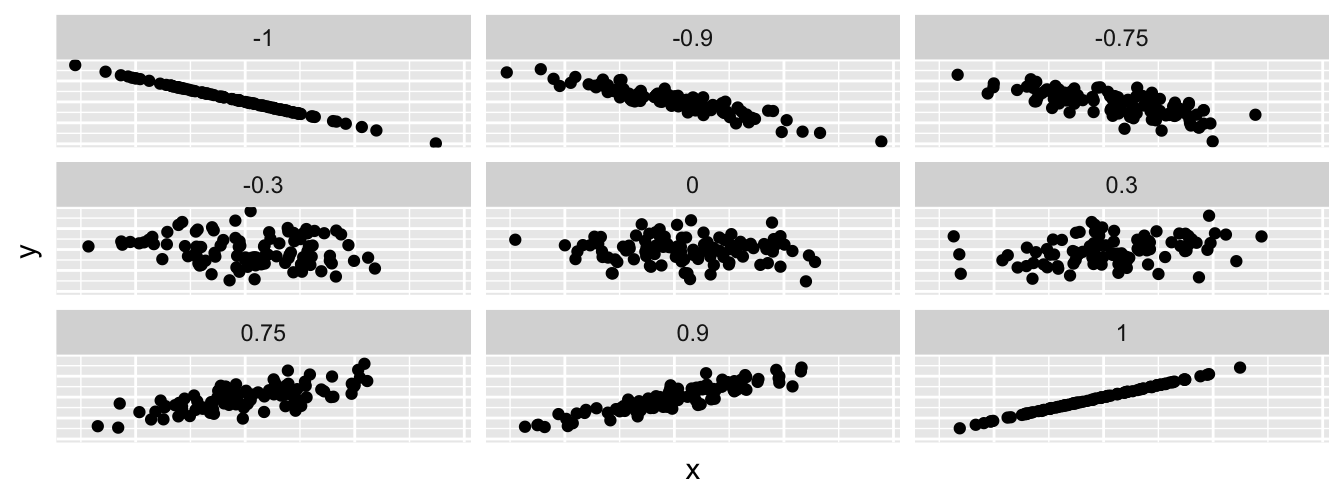
\includegraphics[width=0.9\linewidth,height=0.45\textheight]{week4_2} \end{center}
\end{frame}

\begin{frame}[fragile]{Correlation coefficien: GPA Example}
\protect\hypertarget{correlation-coefficien-gpa-example}{}
Following are the high school GPAs and the college GPAs at the end of
the freshman year for ten different students from the \texttt{Gpa} data
set of the \texttt{BSDA} package.

\normalsize

\begin{Shaded}
\begin{Highlighting}[]
\FunctionTok{library}\NormalTok{(BSDA) }
\FunctionTok{head}\NormalTok{(Gpa)}
\end{Highlighting}
\end{Shaded}

\begin{verbatim}
# A tibble: 6 x 2
  hsgpa collgpa
  <dbl>   <dbl>
1   2.7     2.2
2   3.1     2.8
3   2.1     2.4
4   3.2     3.8
5   2.4     1.9
6   3.4     3.5
\end{verbatim}

\normalsize
\end{frame}

\begin{frame}[fragile]{Correlation coefficient: GPA Example}
\protect\hypertarget{correlation-coefficient-gpa-example}{}
\normalsize

\begin{Shaded}
\begin{Highlighting}[]
\FunctionTok{ggplot}\NormalTok{(}\AttributeTok{data =}\NormalTok{ Gpa, }\FunctionTok{aes}\NormalTok{(}\AttributeTok{x =}\NormalTok{ hsgpa, }\AttributeTok{y =}\NormalTok{ collgpa)) }\SpecialCharTok{+} 
  \FunctionTok{labs}\NormalTok{(}\AttributeTok{x =} \StringTok{"High School GPA"}\NormalTok{, }\AttributeTok{y =} \StringTok{"College GPA"}\NormalTok{) }\SpecialCharTok{+}
  \FunctionTok{geom\_point}\NormalTok{(}\AttributeTok{size =} \DecValTok{5}\NormalTok{, }\AttributeTok{color =} \StringTok{"blue"}\NormalTok{) }\SpecialCharTok{+} 
  \FunctionTok{theme\_bw}\NormalTok{()}
\end{Highlighting}
\end{Shaded}

\begin{center}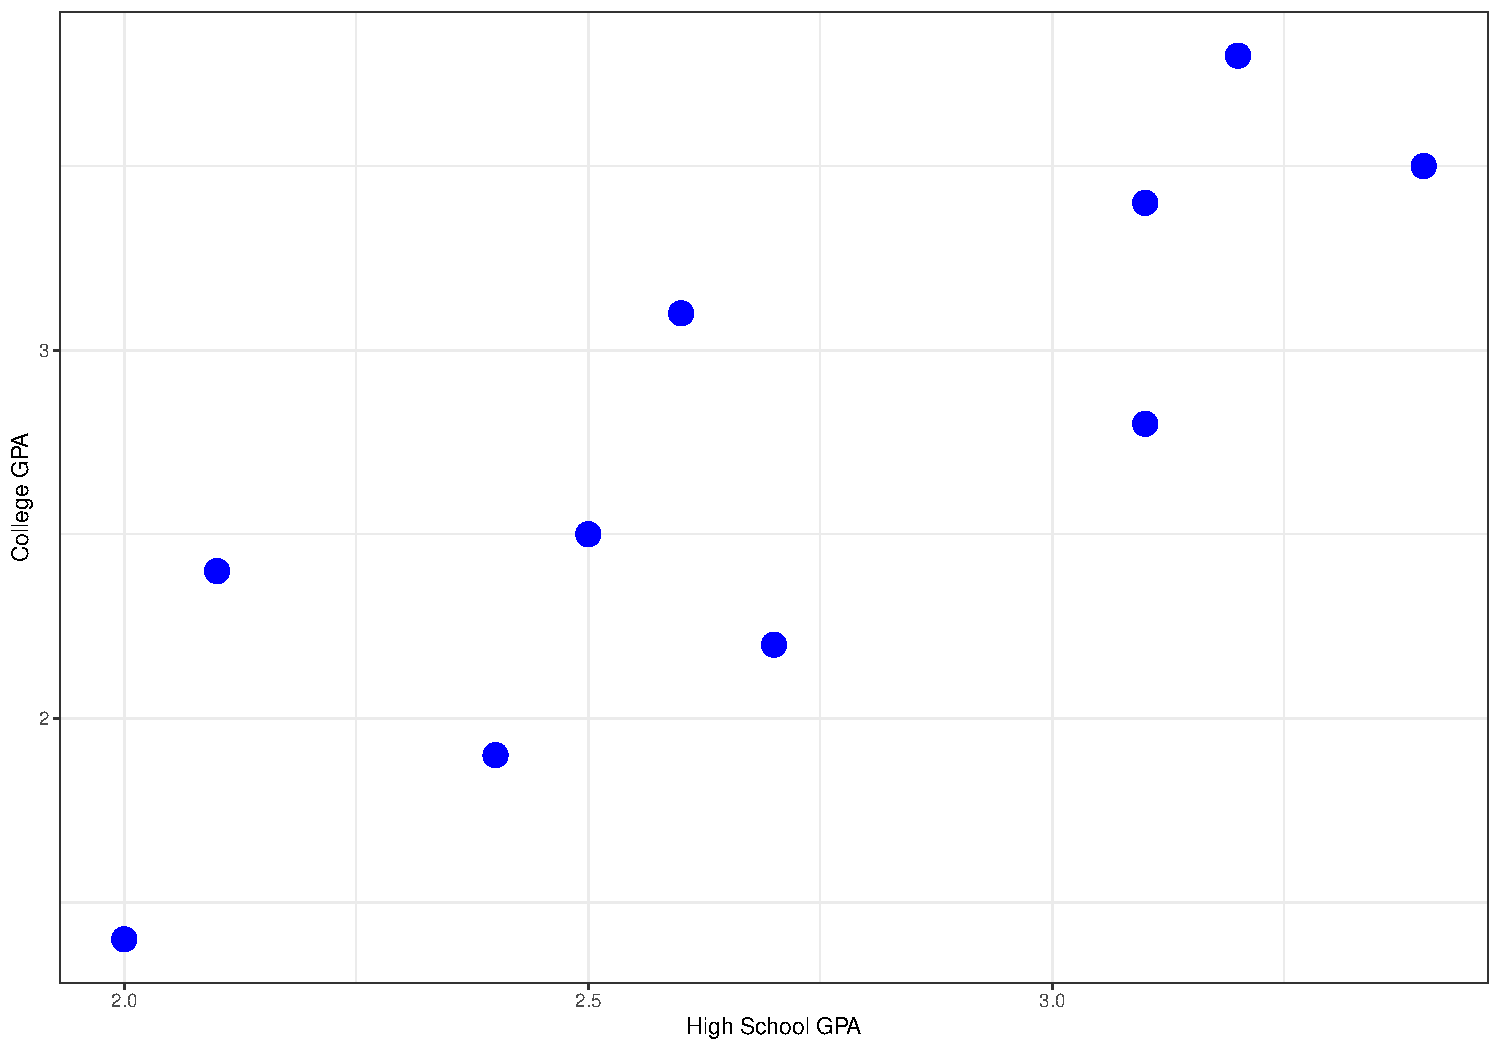
\includegraphics[width=0.5\linewidth,height=0.5\textheight]{Week4_Int_Lect_files/figure-beamer/unnamed-chunk-8-1} \end{center}
\normalsize

The scatterplot shows that the college GPA increases as the high school
GPA increases
\end{frame}

\begin{frame}[fragile]{Correlation coefficien: GPA Example}
\protect\hypertarget{correlation-coefficien-gpa-example-1}{}
\small

\begin{Shaded}
\begin{Highlighting}[]
\NormalTok{values }\OtherTok{\textless{}{-}}\NormalTok{ Gpa }\SpecialCharTok{|\textgreater{}} 
  \FunctionTok{mutate}\NormalTok{(}\AttributeTok{y\_ybar =}\NormalTok{ collgpa }\SpecialCharTok{{-}} \FunctionTok{mean}\NormalTok{(collgpa), }
         \AttributeTok{x\_xbar =}\NormalTok{ hsgpa }\SpecialCharTok{{-}} \FunctionTok{mean}\NormalTok{(hsgpa),}
         \AttributeTok{zx =}\NormalTok{ x\_xbar}\SpecialCharTok{/}\FunctionTok{sd}\NormalTok{(hsgpa), }\AttributeTok{zy =}\NormalTok{ y\_ybar}\SpecialCharTok{/}\FunctionTok{sd}\NormalTok{(collgpa))}
\NormalTok{values}
\end{Highlighting}
\end{Shaded}

\begin{verbatim}
# A tibble: 10 x 6
   hsgpa collgpa y_ybar  x_xbar      zx     zy
   <dbl>   <dbl>  <dbl>   <dbl>   <dbl>  <dbl>
 1   2.7     2.2 -0.5   -0.0100 -0.0210 -0.657
 2   3.1     2.8  0.100  0.39    0.817   0.131
 3   2.1     2.4 -0.300 -0.61   -1.28   -0.394
 4   3.2     3.8  1.1    0.49    1.03    1.44 
 5   2.4     1.9 -0.8   -0.31   -0.650  -1.05 
 6   3.4     3.5  0.8    0.69    1.45    1.05 
 7   2.6     3.1  0.4   -0.110  -0.231   0.525
 8   2       1.4 -1.3   -0.71   -1.49   -1.71 
 9   3.1     3.4  0.7    0.39    0.817   0.919
10   2.5     2.5 -0.200 -0.21   -0.440  -0.263
\end{verbatim}

\normalsize

\[r=\frac{1}{(n-1)}\sum_{i=1}^n \left(\frac{x_i-\bar{x}}{s_x}\right)\left(\frac{y_i-\bar{y}}{s_y}\right)=\frac{\sum z_x z_y}{n-1}\]
\end{frame}

\begin{frame}[fragile]{Correlation coefficient: GPA Example}
\protect\hypertarget{correlation-coefficient-gpa-example-1}{}
\normalsize

\begin{Shaded}
\begin{Highlighting}[]
\NormalTok{values }\SpecialCharTok{|\textgreater{}} 
  \FunctionTok{summarize}\NormalTok{(}\AttributeTok{r =}\NormalTok{ (}\DecValTok{1}\SpecialCharTok{/}\DecValTok{9}\NormalTok{)}\SpecialCharTok{*}\FunctionTok{sum}\NormalTok{(zx}\SpecialCharTok{*}\NormalTok{zy))}
\end{Highlighting}
\end{Shaded}

\begin{verbatim}
# A tibble: 1 x 1
      r
  <dbl>
1 0.844
\end{verbatim}

\normalsize

Using the build in \texttt{cor()} function:

\normalsize

\begin{Shaded}
\begin{Highlighting}[]
\NormalTok{Gpa }\SpecialCharTok{|\textgreater{}} 
  \FunctionTok{summarize}\NormalTok{(}\AttributeTok{r =} \FunctionTok{cor}\NormalTok{(collgpa, hsgpa))}
\end{Highlighting}
\end{Shaded}

\begin{verbatim}
# A tibble: 1 x 1
      r
  <dbl>
1 0.844
\end{verbatim}

\normalsize
\end{frame}

\begin{frame}[fragile]{Correlation coefficient: GPA Example}
\protect\hypertarget{correlation-coefficient-gpa-example-2}{}
Using \texttt{get\_correlation()} function in the \texttt{moderndive}
package.

\normalsize

\begin{Shaded}
\begin{Highlighting}[]
\NormalTok{Gpa }\SpecialCharTok{|\textgreater{}} 
  \FunctionTok{get\_correlation}\NormalTok{(}\AttributeTok{formula =}\NormalTok{ collgpa }\SpecialCharTok{\textasciitilde{}}\NormalTok{ hsgpa)}
\end{Highlighting}
\end{Shaded}

\begin{verbatim}
# A tibble: 1 x 1
    cor
  <dbl>
1 0.844
\end{verbatim}

\normalsize
\end{frame}

\begin{frame}[fragile]{Correlation coefficient: GPA Example}
\protect\hypertarget{correlation-coefficient-gpa-example-3}{}
\normalsize

\begin{Shaded}
\begin{Highlighting}[]
\NormalTok{p1 }\OtherTok{\textless{}{-}} \FunctionTok{ggplot}\NormalTok{(}\AttributeTok{data =}\NormalTok{ Gpa, }\FunctionTok{aes}\NormalTok{(}\AttributeTok{x =}\NormalTok{ hsgpa, }\AttributeTok{y =}\NormalTok{ collgpa)) }\SpecialCharTok{+} 
  \FunctionTok{geom\_point}\NormalTok{(}\AttributeTok{size =} \DecValTok{5}\NormalTok{, }\AttributeTok{color =} \StringTok{"red"}\NormalTok{) }\SpecialCharTok{+} 
  \FunctionTok{theme\_bw}\NormalTok{()}
\NormalTok{p2 }\OtherTok{\textless{}{-}} \FunctionTok{ggplot}\NormalTok{(}\AttributeTok{data =}\NormalTok{ values, }\FunctionTok{aes}\NormalTok{(}\AttributeTok{x =}\NormalTok{ zx, }\AttributeTok{y =}\NormalTok{ zy)) }\SpecialCharTok{+} 
  \FunctionTok{geom\_point}\NormalTok{(}\AttributeTok{size =} \DecValTok{5}\NormalTok{, }\AttributeTok{color =} \StringTok{"blue"}\NormalTok{) }\SpecialCharTok{+} 
  \FunctionTok{theme\_bw}\NormalTok{()}
\FunctionTok{library}\NormalTok{(patchwork)}
\NormalTok{p1}\SpecialCharTok{/}\NormalTok{p2}
\end{Highlighting}
\end{Shaded}

\begin{center}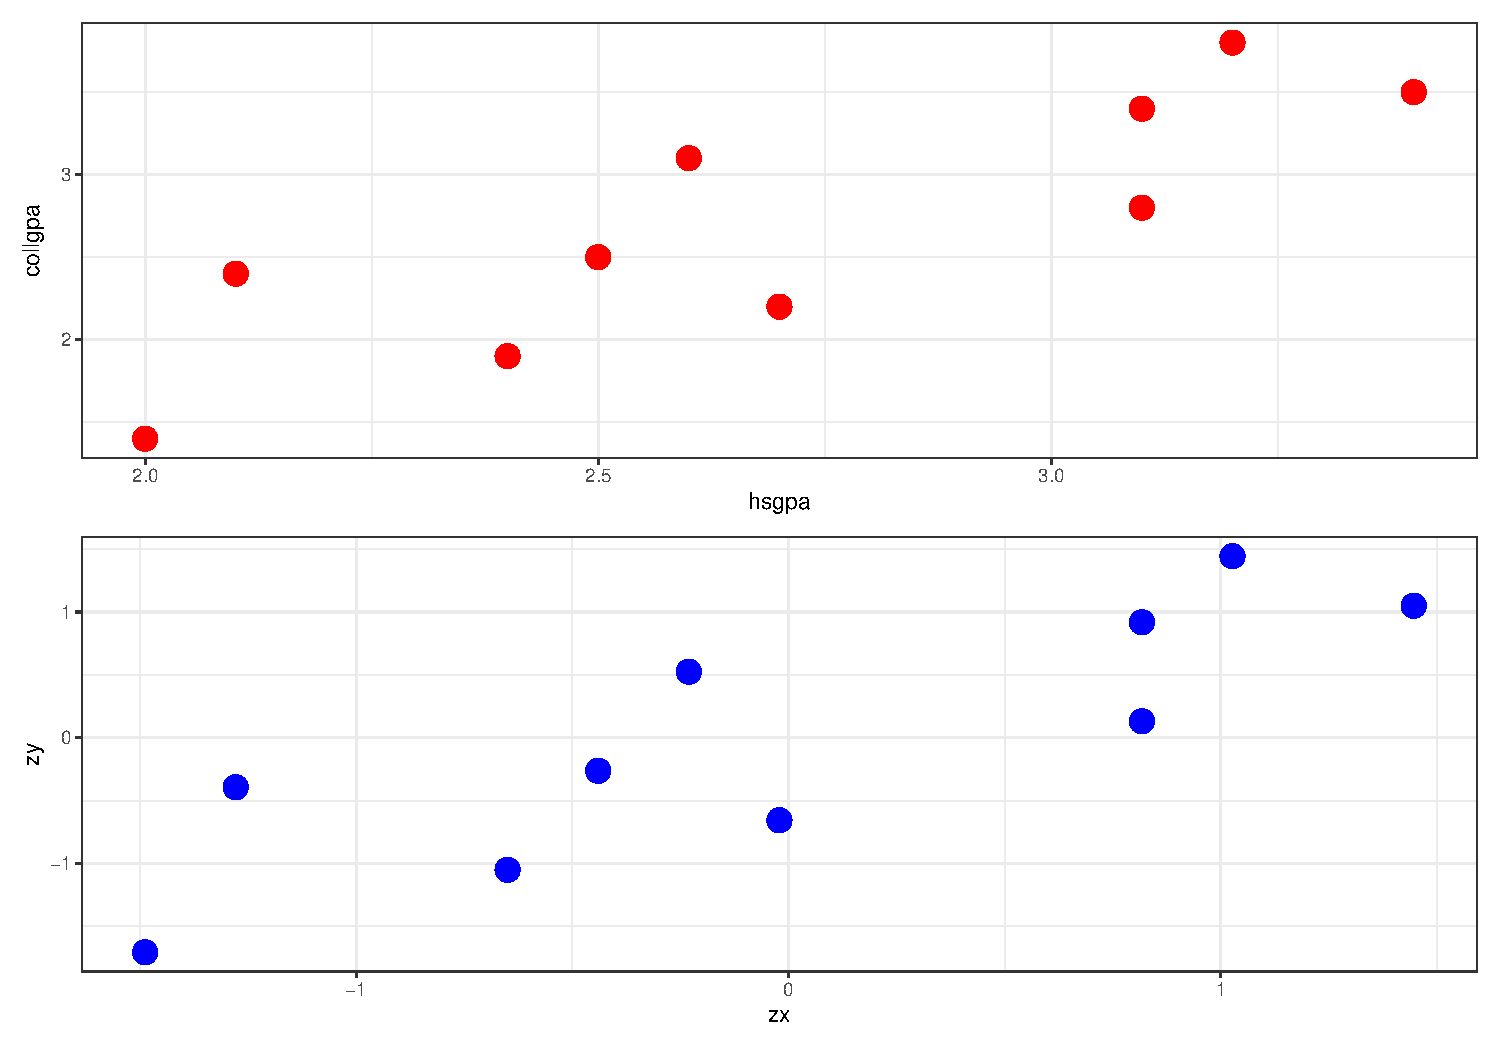
\includegraphics[width=0.6\linewidth,height=0.45\textheight]{Week4_Int_Lect_files/figure-beamer/unnamed-chunk-13-1} \end{center}
\normalsize
\end{frame}

\begin{frame}[fragile]{Correlation coefficient: Teaching Evaluations
Example}
\protect\hypertarget{correlation-coefficient-teaching-evaluations-example}{}
\normalsize

\begin{Shaded}
\begin{Highlighting}[]
\NormalTok{evals\_ch5 }\SpecialCharTok{|\textgreater{}} 
  \FunctionTok{get\_correlation}\NormalTok{(}\AttributeTok{formula =}\NormalTok{ score }\SpecialCharTok{\textasciitilde{}}\NormalTok{ bty\_avg)}
\end{Highlighting}
\end{Shaded}

\begin{verbatim}
# A tibble: 1 x 1
    cor
  <dbl>
1 0.187
\end{verbatim}

\normalsize

\normalsize

\begin{Shaded}
\begin{Highlighting}[]
\NormalTok{evals\_ch5 }\SpecialCharTok{|\textgreater{}} 
  \FunctionTok{summarize}\NormalTok{(}\AttributeTok{correlation =} \FunctionTok{cor}\NormalTok{(score, bty\_avg))}
\end{Highlighting}
\end{Shaded}

\begin{verbatim}
# A tibble: 1 x 1
  correlation
        <dbl>
1       0.187
\end{verbatim}

\normalsize
\end{frame}

\begin{frame}[fragile]{Step 3: create data visualizations}
\protect\hypertarget{step-3-create-data-visualizations}{}
\normalsize

\begin{Shaded}
\begin{Highlighting}[]
\FunctionTok{ggplot}\NormalTok{(evals\_ch5, }\FunctionTok{aes}\NormalTok{(}\AttributeTok{x =}\NormalTok{ bty\_avg, }\AttributeTok{y =}\NormalTok{ score)) }\SpecialCharTok{+}
  \FunctionTok{geom\_jitter}\NormalTok{(}\AttributeTok{size =} \DecValTok{3}\NormalTok{, }\AttributeTok{color =} \StringTok{"blue"}\NormalTok{) }\SpecialCharTok{+}
  \FunctionTok{labs}\NormalTok{(}\AttributeTok{x =} \StringTok{"Beauty Score"}\NormalTok{, }\AttributeTok{y =} \StringTok{"Teaching Score"}\NormalTok{,}
       \AttributeTok{title =} \StringTok{"Scatterplot teaching and beauty scores"}\NormalTok{) }\SpecialCharTok{+}
  \FunctionTok{theme\_bw}\NormalTok{()}
\end{Highlighting}
\end{Shaded}

\begin{center}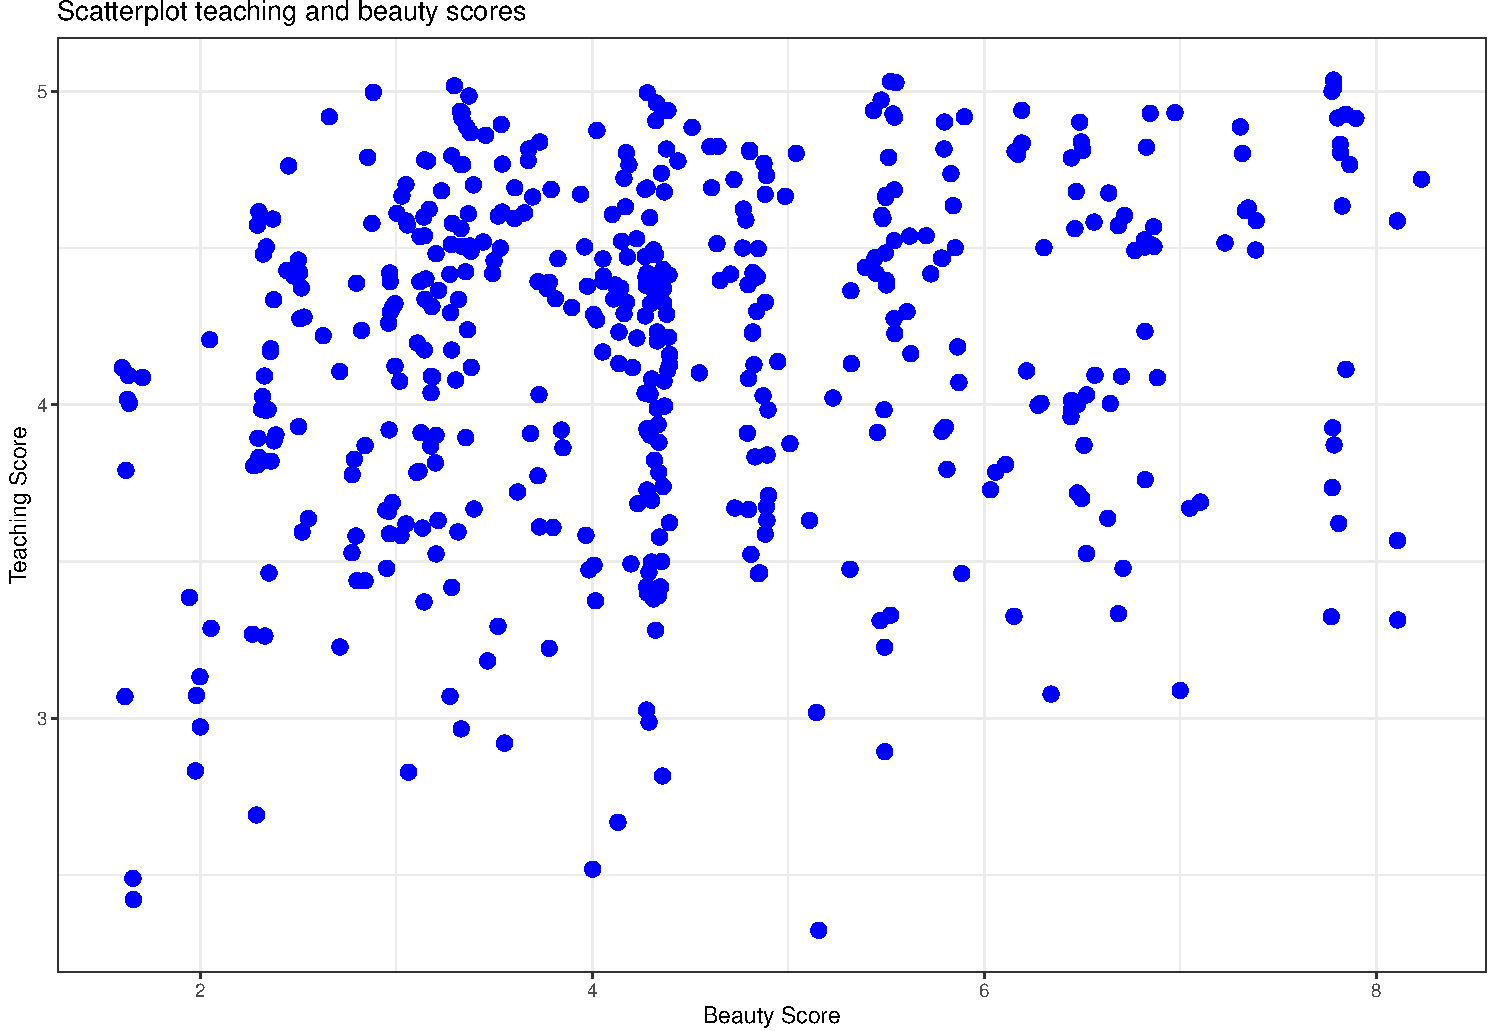
\includegraphics[width=0.6\linewidth,height=0.45\textheight]{Week4_Int_Lect_files/figure-beamer/unnamed-chunk-16-1} \end{center}
\normalsize
\end{frame}

\begin{frame}[fragile]{Step 3: creating data visualizations}
\protect\hypertarget{step-3-creating-data-visualizations}{}
Add ``best-fitting'' line (regression line).

\tiny

\begin{Shaded}
\begin{Highlighting}[]
\FunctionTok{ggplot}\NormalTok{(evals\_ch5, }\FunctionTok{aes}\NormalTok{(}\AttributeTok{x =}\NormalTok{ bty\_avg, }\AttributeTok{y =}\NormalTok{ score)) }\SpecialCharTok{+}
  \FunctionTok{geom\_point}\NormalTok{(}\AttributeTok{size =} \DecValTok{3}\NormalTok{, }\AttributeTok{color =} \StringTok{"purple"}\NormalTok{) }\SpecialCharTok{+}
  \FunctionTok{labs}\NormalTok{(}\AttributeTok{x =} \StringTok{"Beauty Score"}\NormalTok{, }\AttributeTok{y =} \StringTok{"Teaching Score"}\NormalTok{,}
       \AttributeTok{title =} \StringTok{"Teaching and Beauty Scores"}\NormalTok{) }\SpecialCharTok{+}  
  \FunctionTok{geom\_smooth}\NormalTok{(}\AttributeTok{method =} \StringTok{"lm"}\NormalTok{, }\AttributeTok{se =} \ConstantTok{FALSE}\NormalTok{) }\SpecialCharTok{+} 
  \FunctionTok{theme\_bw}\NormalTok{()}
\end{Highlighting}
\end{Shaded}

\begin{center}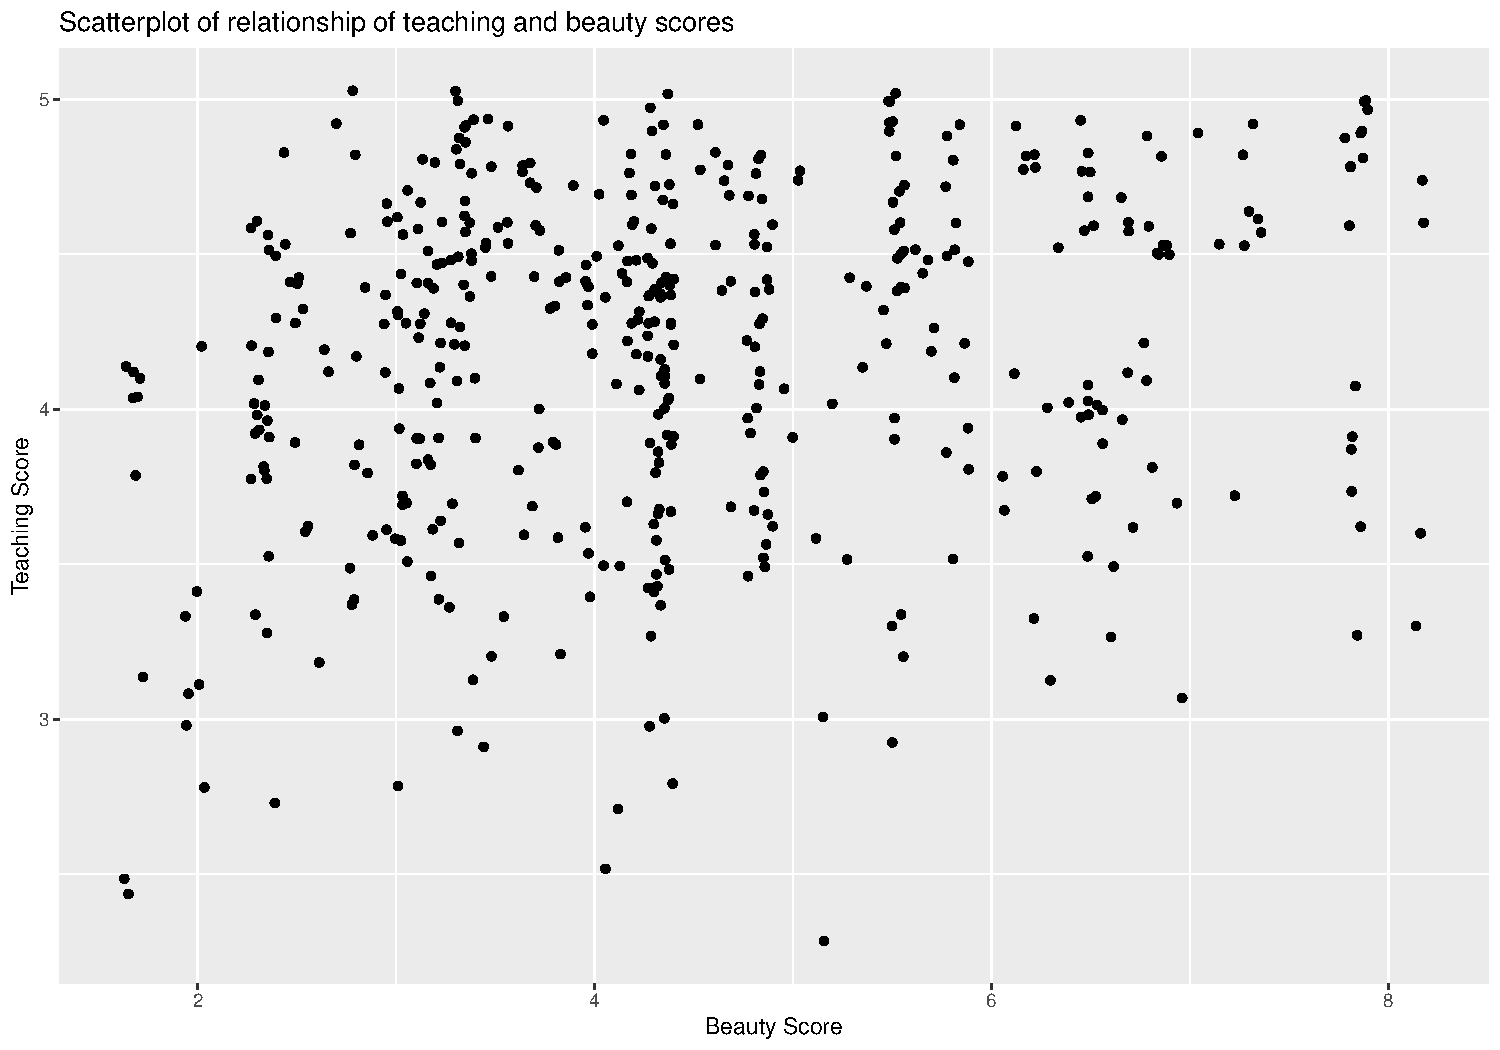
\includegraphics[width=0.6\linewidth,height=0.45\textheight]{Week4_Int_Lect_files/figure-beamer/unnamed-chunk-17-1} \end{center}
\normalsize
\end{frame}

\hypertarget{simple-linear-regression}{%
\section{Simple linear regression}\label{simple-linear-regression}}

\begin{frame}{Simple linear regression}
\protect\hypertarget{simple-linear-regression-1}{}
You may recall from secondary/high school algebra that the equation of a
line is: \[y=m\cdot x + b\]

\begin{itemize}
\item
  The intercept coefficient is \(b\) is the value of \(y\) when \(x=0\).
\item
  The slope coefficient \(m\) for \(x\) is the increase in \(y\) for
  every increase in \(x\).
\end{itemize}

However, when defining regression equation line, we use slightly
different notation.
\end{frame}

\begin{frame}{Simple linear regression}
\protect\hypertarget{simple-linear-regression-2}{}
The regression equation is given by: \[y=\beta_0+\beta_1x+\epsilon\]

\begin{itemize}
\item
  where \(\beta_0\) is the intercept,
\item
  \(\beta_1\) is the slope,
\item
  and \(\epsilon\) is random error.
\item
  For the \(i\)th trial, we have:
\end{itemize}

\[y_i=\beta_0+\beta_1x_i+\epsilon_i\]
\end{frame}

\begin{frame}{Simple linear regression}
\protect\hypertarget{simple-linear-regression-3}{}
The line that best fits the data is given by, \[\hat{y}=b_0+b_1x\] where
\(b_0\) and \(b_1\) are estimates for the population parameters
\(\beta_0\) and \(\beta_1\).

\begin{itemize}
\item
  From the best fit line, we can compute the:

  \begin{itemize}
  \tightlist
  \item
    predicted \(\hat{y}\) for each \(x\) and
  \item
    measure the error of prediction.
  \end{itemize}
\item
  The error of prediction, \(e_i\) (also called residual) is the
  difference in the actual \(y_i\) and the predicted \(\hat{y}_i\).
  \[e_i=y_i-\hat{y}_i.\]
\end{itemize}
\end{frame}

\begin{frame}{The least squares regression line}
\protect\hypertarget{the-least-squares-regression-line}{}
The least squares regression line is:

\[\hat{y}=b_0+b_1x\]

where
\[b_1=\frac{\sum(x_i-\bar{x})(y_i-\bar{y})}{\sum(x_i-\bar{x})^2}=r \frac{s_y}{s_x}\]
and \[b_0=\bar{y}-b_1\bar{x}.\]
\end{frame}

\begin{frame}[fragile]{Regression: Teaching Evaluations Example}
\protect\hypertarget{regression-teaching-evaluations-example}{}
\begin{center}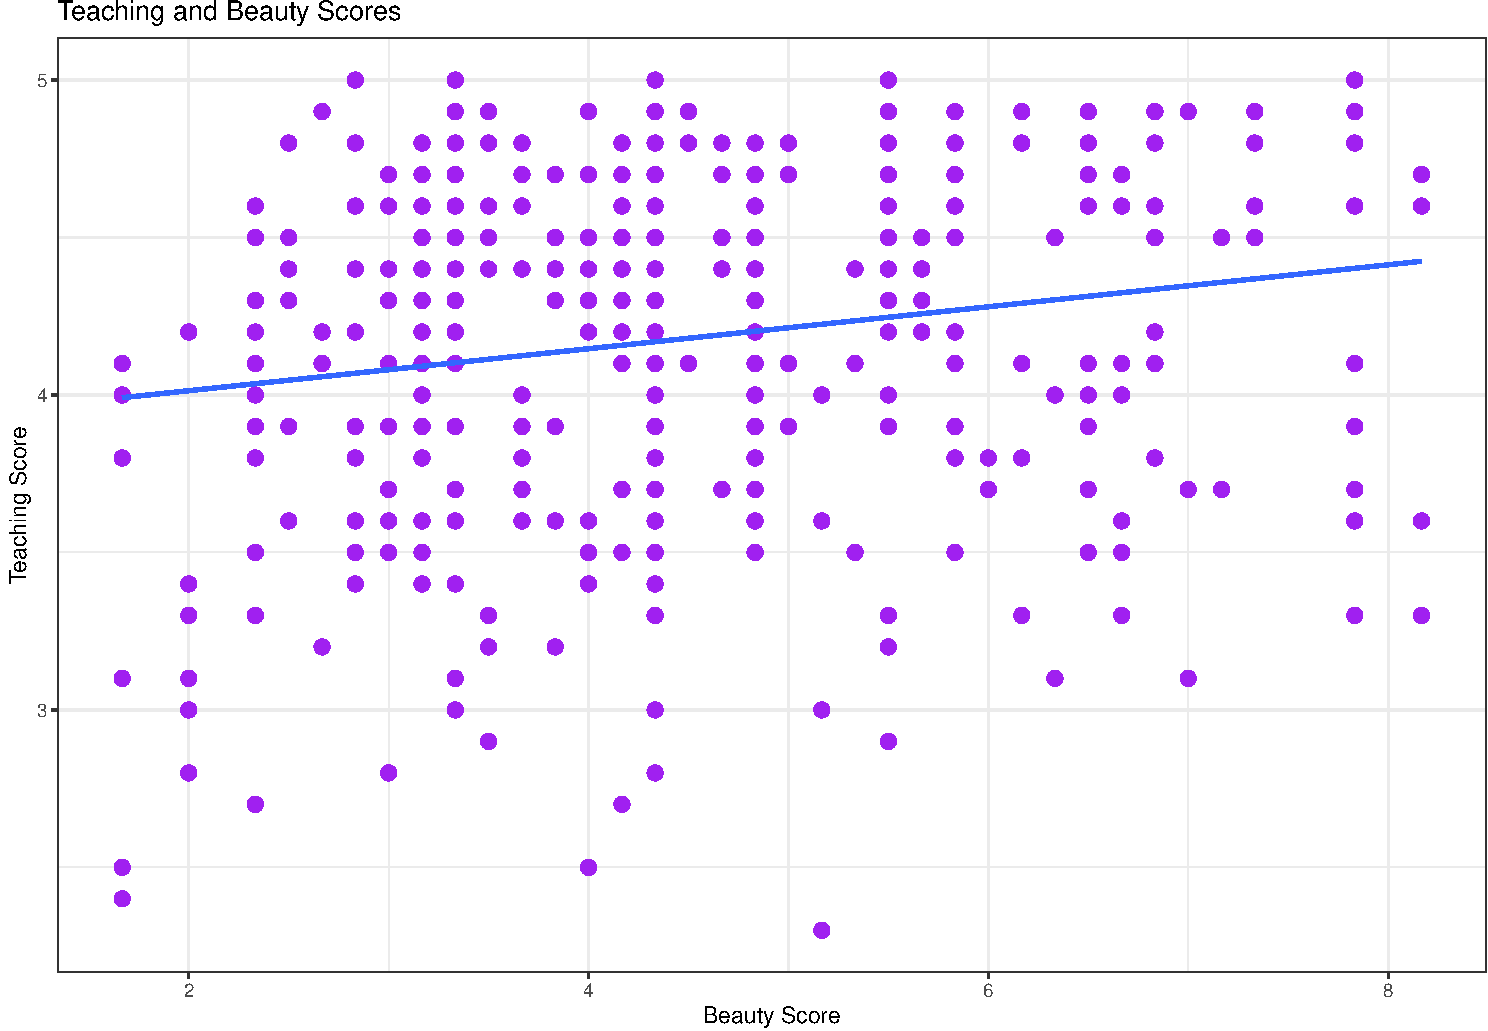
\includegraphics[width=0.6\linewidth,height=0.45\textheight]{Week4_Int_Lect_files/figure-beamer/unnamed-chunk-18-1} \end{center}

\begin{itemize}
\item
  We know that the regression line has a positive slope \(b_1\)
  corresponding to our explanatory \(x\) variable \texttt{bty\_avg}.
\item
  However, what is the numerical value of the slope \(b_1\)? What about
  the intercept \(b_0\)?
\end{itemize}
\end{frame}

\begin{frame}[fragile]{Regression: Teaching Evaluations Example}
\protect\hypertarget{regression-teaching-evaluations-example-1}{}
We obtain the regression line parameters in two steps:

\begin{enumerate}
\item
  We ``fit'' the linear regression model using the \texttt{lm()}
  function and save it, lets call it \texttt{score\_model}.
\item
  We get the regression table by applying the
  \texttt{get\_regression\_table()} function from the
  \texttt{moderndive} package to \texttt{score\_model} or using
  \texttt{summary()} on the linear model object.
\end{enumerate}
\end{frame}

\begin{frame}[fragile]{Regression: Teaching Evaluations Example}
\protect\hypertarget{regression-teaching-evaluations-example-2}{}
\small

\begin{Shaded}
\begin{Highlighting}[]
\CommentTok{\# Fit regression model:}
\NormalTok{score\_model }\OtherTok{\textless{}{-}} \FunctionTok{lm}\NormalTok{(score }\SpecialCharTok{\textasciitilde{}}\NormalTok{ bty\_avg, }\AttributeTok{data =}\NormalTok{ evals\_ch5)}
\CommentTok{\# Get regression table:}
\FunctionTok{get\_regression\_table}\NormalTok{(score\_model)}
\end{Highlighting}
\end{Shaded}

\begin{verbatim}
# A tibble: 2 x 7
  term      estimate std_error statistic p_value lower_ci upper_ci
  <chr>        <dbl>     <dbl>     <dbl>   <dbl>    <dbl>    <dbl>
1 intercept    3.88      0.076     51.0        0    3.73     4.03 
2 bty_avg      0.067     0.016      4.09       0    0.035    0.099
\end{verbatim}
\end{frame}

\begin{frame}[fragile]{Regression: Teaching Evaluations Example}
\protect\hypertarget{regression-teaching-evaluations-example-3}{}
\small

\begin{Shaded}
\begin{Highlighting}[]
\CommentTok{\# Using summary()}
\FunctionTok{summary}\NormalTok{(score\_model)}
\end{Highlighting}
\end{Shaded}

\begin{verbatim}

Call:
lm(formula = score ~ bty_avg, data = evals_ch5)

Residuals:
    Min      1Q  Median      3Q     Max 
-1.9246 -0.3690  0.1420  0.3977  0.9309 

Coefficients:
            Estimate Std. Error t value Pr(>|t|)    
(Intercept)  3.88034    0.07614   50.96  < 2e-16 ***
bty_avg      0.06664    0.01629    4.09 5.08e-05 ***
---
Signif. codes:  0 '***' 0.001 '**' 0.01 '*' 0.05 '.' 0.1 ' ' 1

Residual standard error: 0.5348 on 461 degrees of freedom
Multiple R-squared:  0.03502,   Adjusted R-squared:  0.03293 
F-statistic: 16.73 on 1 and 461 DF,  p-value: 5.083e-05
\end{verbatim}
\end{frame}

\begin{frame}[fragile]{Regression: Teaching Evaluations Example}
\protect\hypertarget{regression-teaching-evaluations-example-4}{}
\small

\begin{Shaded}
\begin{Highlighting}[]
\CommentTok{\# Use formula}
\NormalTok{evals\_ch5 }\SpecialCharTok{|\textgreater{}} 
  \FunctionTok{summarize}\NormalTok{(}\AttributeTok{b1 =} \FunctionTok{cor}\NormalTok{(bty\_avg, score)}\SpecialCharTok{*}\FunctionTok{sd}\NormalTok{(score)}\SpecialCharTok{/}\FunctionTok{sd}\NormalTok{(bty\_avg),}
            \AttributeTok{b0 =} \FunctionTok{mean}\NormalTok{(score) }\SpecialCharTok{{-}}\NormalTok{ b1}\SpecialCharTok{*}\FunctionTok{mean}\NormalTok{(bty\_avg))}
\end{Highlighting}
\end{Shaded}

\begin{verbatim}
# A tibble: 1 x 2
      b1    b0
   <dbl> <dbl>
1 0.0666  3.88
\end{verbatim}
\end{frame}

\begin{frame}[fragile]{Regression: Teaching Evaluations Example}
\protect\hypertarget{regression-teaching-evaluations-example-5}{}
Lets interpret the regression table. The equation of the regression
line:

\[
\begin{aligned}
\hat{y} &= b_0 +b_1\cdot x \\
\widehat{\text{score}} &= b_0 + b_{\text{bty\_avg}}\\
&= 3.88 + 0.067\cdot\text{bty\_avg}
\end{aligned}
\]

\begin{itemize}
\item
  The intercept \(b_0 = 3.88\)

  \begin{itemize}
  \tightlist
  \item
    is the average teaching score \(\hat{y}=\widehat{\text{score}}\) for
    those courses where the instructor had a ``beauty'' score
    (\texttt{bty\_avg}) of 0.
  \item
    Note however that \texttt{bty\_avg} of 0 is impossible since the
    beauty scores ranges from 1 to 10.
  \end{itemize}
\end{itemize}
\end{frame}

\begin{frame}[fragile]{Regression: Teaching Evaluations Example}
\protect\hypertarget{regression-teaching-evaluations-example-6}{}
\begin{itemize}
\item
  The slope \(b_1\) of \texttt{bty\_avg} is 0.067.

  \begin{itemize}
  \tightlist
  \item
    The sign is positive, suggesting a positive relationship between
    these two variables, meaning teachers with higher ``beauty'' scores
    also tend to have higher teaching scores.
  \item
    For every increase of 1 unit in \texttt{bty\_avg}, there is an
    associated increase of, on average, 0.067 units of \texttt{score}.
  \end{itemize}
\end{itemize}
\end{frame}

\begin{frame}[fragile]{Observed/fitted values and residuals}
\protect\hypertarget{observedfitted-values-and-residuals}{}
Now we are interested in information on individual observations. For
example, let's focus on the 21st of the 463 courses in the
\texttt{evals\_ch5} dataframe

\small

\begin{Shaded}
\begin{Highlighting}[]
\CommentTok{\# Fit regression model:}
\NormalTok{evals\_ch5[}\DecValTok{21}\NormalTok{,]}
\end{Highlighting}
\end{Shaded}

\begin{verbatim}
# A tibble: 1 x 4
     ID score bty_avg   age
  <int> <dbl>   <dbl> <int>
1    21   4.9    7.33    31
\end{verbatim}

\begin{Shaded}
\begin{Highlighting}[]
\NormalTok{evals\_ch5[}\DecValTok{21}\NormalTok{,]}\SpecialCharTok{$}\NormalTok{bty\_avg}
\end{Highlighting}
\end{Shaded}

\begin{verbatim}
[1] 7.333
\end{verbatim}

\normalsize

\begin{itemize}
\tightlist
\item
  We want to know what is the value \(\hat{y}\) on the regression line
  corresponding to instructor's \texttt{bty\_avg} ``beauty'' score of
  7.333.
\end{itemize}
\end{frame}

\begin{frame}{Observed/fitted values and residuals}
\protect\hypertarget{observedfitted-values-and-residuals-1}{}
\begin{center}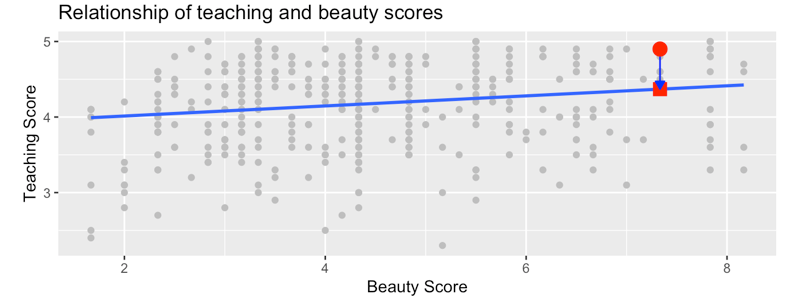
\includegraphics[width=0.8\linewidth,height=0.4\textheight]{week4_4} \end{center}

\begin{itemize}
\tightlist
\item
  Square: The fitted value \(\hat{y}_i\) is given by
  \[\hat{y}_i=b_0+b_1\cdot x=3.88+0.067\cdot 7.333=4.369\]
\item
  Circle: The observed value \(y_i=4.9\).
\item
  Arrow: The length of the arrow is the residual or error and is given
  by \[e_i=y_i-\hat{y}_i=4.9-4.369=0.531.\]
\end{itemize}
\end{frame}

\begin{frame}[fragile]{Observed/fitted values and residuals}
\protect\hypertarget{observedfitted-values-and-residuals-2}{}
To compute both the fitted value and residual for all observations in
the data we use the \texttt{get\_regression\_points()} function.

\small

\begin{Shaded}
\begin{Highlighting}[]
\NormalTok{regression\_points }\OtherTok{\textless{}{-}} \FunctionTok{get\_regression\_points}\NormalTok{(score\_model)}
\NormalTok{regression\_points}
\end{Highlighting}
\end{Shaded}

\begin{verbatim}
# A tibble: 463 x 5
      ID score bty_avg score_hat residual
   <int> <dbl>   <dbl>     <dbl>    <dbl>
 1     1   4.7    5         4.21    0.486
 2     2   4.1    5         4.21   -0.114
 3     3   3.9    5         4.21   -0.314
 4     4   4.8    5         4.21    0.586
 5     5   4.6    3         4.08    0.52 
 6     6   4.3    3         4.08    0.22 
 7     7   2.8    3         4.08   -1.28 
 8     8   4.1    3.33      4.10   -0.002
 9     9   3.4    3.33      4.10   -0.702
10    10   4.5    3.17      4.09    0.409
# i 453 more rows
\end{verbatim}

\normalsize
\end{frame}

\begin{frame}{Assessing the fit}
\protect\hypertarget{assessing-the-fit}{}
\begin{itemize}
\item
  The regression model is a good model if the scatterplot of residuals
  versus \(x\)-values or if the scatterplot of residuals versus
  \(\hat{y}\)-values has no interesting features.

  \begin{itemize}
  \tightlist
  \item
    No direction
  \item
    No shape
  \item
    No bends
  \item
    No outliers
  \item
    No identifiable pattern
  \item
    Equal or constant variance (homoscedasticity)
  \end{itemize}
\item
  In addition, for a good model, the residuals are approximately
  normally distributed. Check the histogram of residuals.
\end{itemize}
\end{frame}

\begin{frame}{Assessing the fit}
\protect\hypertarget{assessing-the-fit-1}{}
\begin{center}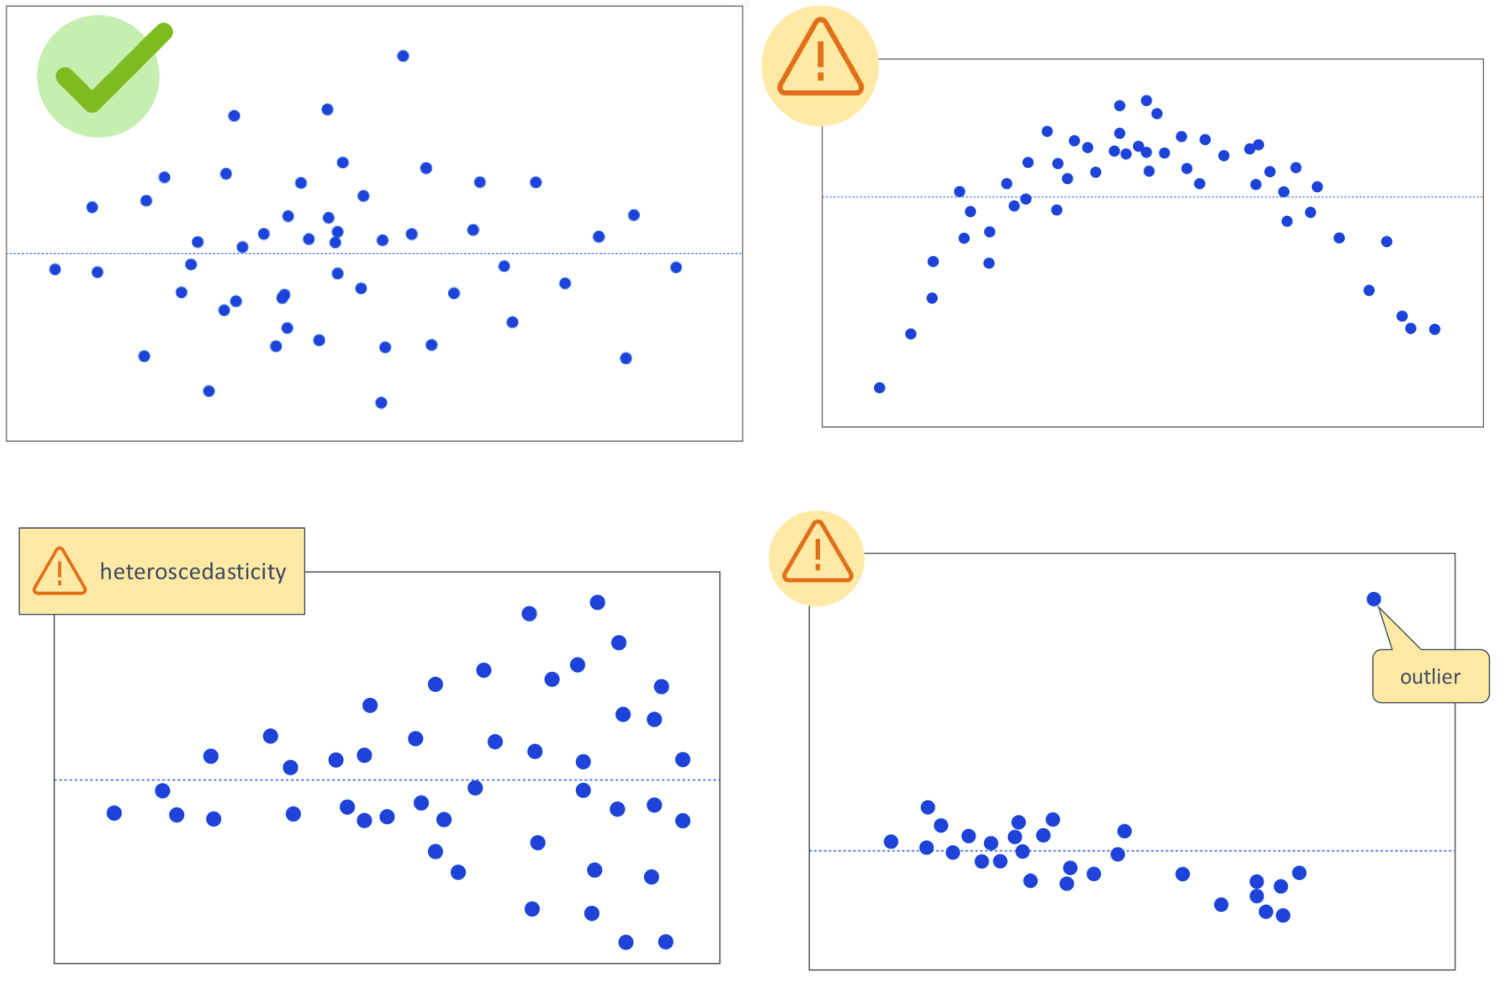
\includegraphics[width=0.9\linewidth]{Week4_Int_Lect_files/figure-beamer/unnamed-chunk-25-1} \end{center}
\end{frame}

\begin{frame}[fragile]{Assessing the fit: Teaching Evaluations Example}
\protect\hypertarget{assessing-the-fit-teaching-evaluations-example}{}
\normalsize

\begin{Shaded}
\begin{Highlighting}[]
\FunctionTok{library}\NormalTok{(ggfortify)}
\FunctionTok{autoplot}\NormalTok{(score\_model, }\AttributeTok{ncol =} \DecValTok{2}\NormalTok{, }\AttributeTok{nrow =} \DecValTok{1}\NormalTok{, }\AttributeTok{which =} \DecValTok{1}\SpecialCharTok{:}\DecValTok{2}\NormalTok{) }\SpecialCharTok{+}
  \FunctionTok{theme\_bw}\NormalTok{()}
\end{Highlighting}
\end{Shaded}

\begin{center}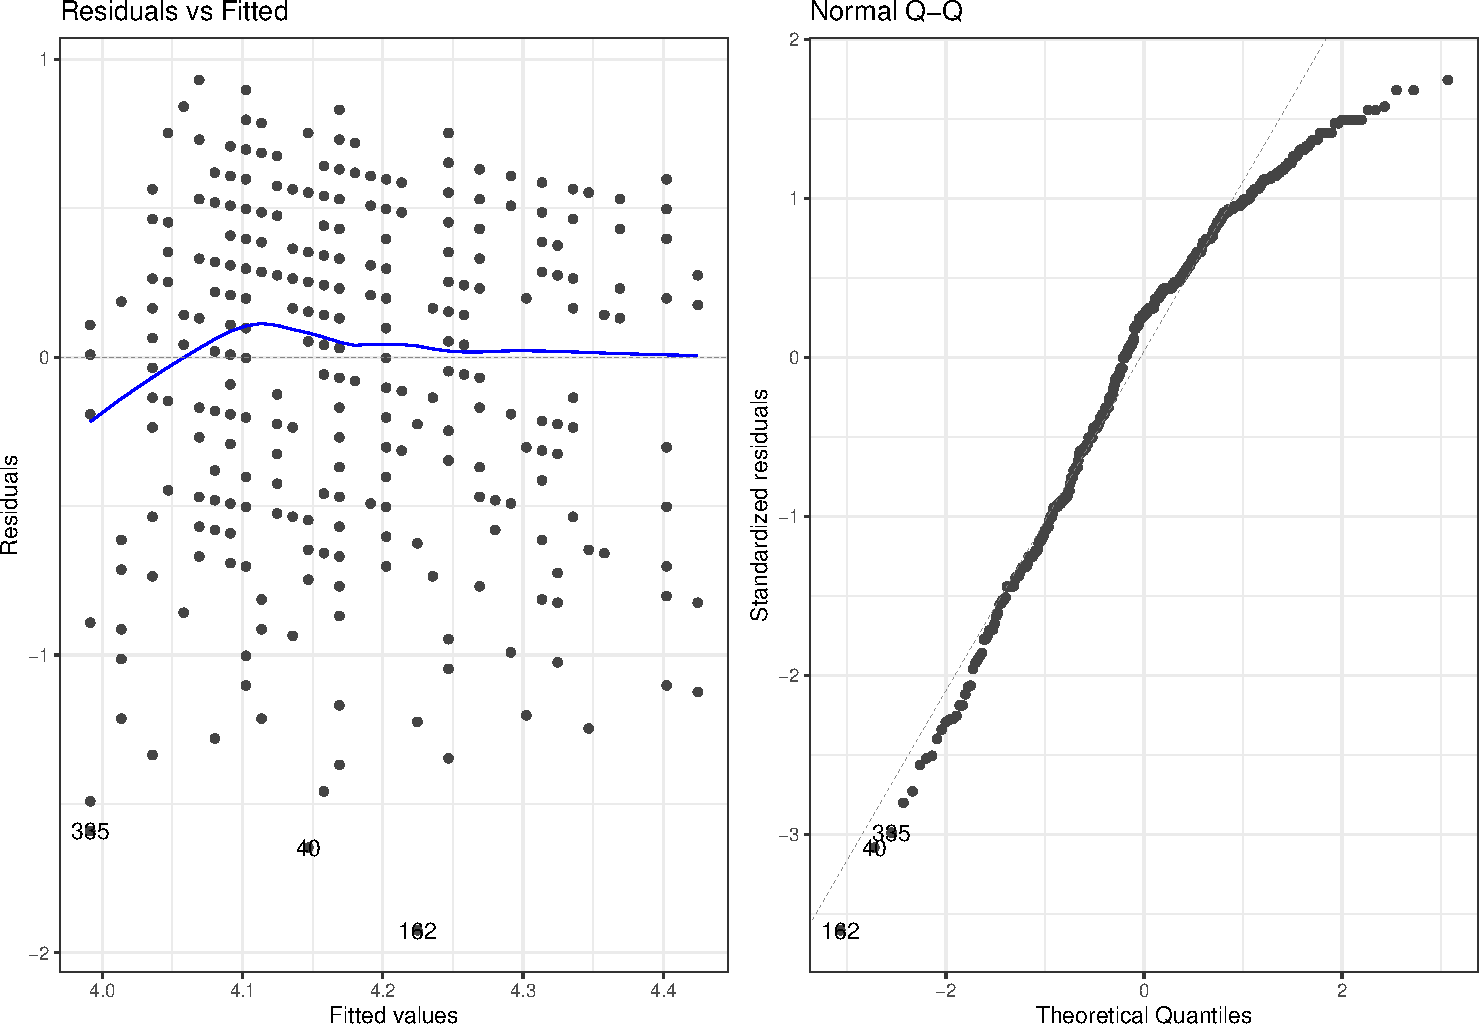
\includegraphics[width=0.8\linewidth,height=0.6\textheight]{Week4_Int_Lect_files/figure-beamer/unnamed-chunk-26-1} \end{center}
\normalsize
\end{frame}

\hypertarget{confidence-intervals-and-tests}{%
\section{Confidence Intervals and
Tests}\label{confidence-intervals-and-tests}}

\begin{frame}{Estimating \(\sigma^2\)}
\protect\hypertarget{estimating-sigma2}{}
The regression equations give the mean of the group. What is the
standard deviation of this group? That is, we have to estimate
\(\sigma\).
\[ y_i=\beta_0+\beta_1x_i+\epsilon_i, \quad \quad Var(\epsilon_i)=\sigma^2.\]
A natural estimator for \(\sigma^2\) is:
\[\frac{1}{n}\sum_{i=1}^n(\epsilon_i-E(\epsilon))^2=\frac{1}{n}\sum_{i=1}^n(\epsilon_i)^2=\frac{1}{n}\sum_{i=1}^n(y_i-\beta_0-\beta_1x_i)^2.\]
Since, \(\beta_0\) and \(\beta_1\) are unknown, we use the estimators:
\[ \frac{1}{n}\sum_{i=1}^ne_i^2=\frac{1}{n}\sum_{i=1}^n(y_i-b_0-b_1x_i)^2=\frac{SSE}{n}\]
\end{frame}

\begin{frame}{Estimating \(\sigma^2\)}
\protect\hypertarget{estimating-sigma2-1}{}
Since \(b_0\), \(b_1\) are estimators, the \(\hat{e}_i^2\) are not
independent. We use the following estimator of \(\sigma^2\):
\[ s^2=\frac{SSE}{n-2}=MSE,\] where \(n-2\) is the degree of freedom
(df) (why?), and MSE stands for error mean square or residual mean
square. Generally, \(df=\text{number of cases - number of parameters}\).

\begin{itemize}
\tightlist
\item
  The residual standard error, \(s=\sqrt{MSE}\), gives the average error
  the model predicts.
\end{itemize}
\end{frame}

\begin{frame}{Properties of OLS}
\protect\hypertarget{properties-of-ols}{}
If we assume that \(\epsilon_i \sim N(0, \sigma^2)\), then the OLS
estimates are also maximum likelihood estimates (MLE). Under the normal
assumption,
\[b_1\sim N\left(\beta_1 , \frac{\sigma^2}{\sum(x_i-\bar{x})^2}\right),\]
\[b_0\sim N\left(\beta_0 , \sigma^2\left(\frac{1}{n}+\frac{\bar{x}^2}{\sum(x_i-\bar{x})^2}\right)\right),\]
These quantities will be used to construct confidence intervals, to
perform hypothesis testing, and to make other statistical inferences.
\end{frame}

\begin{frame}{Confidence Intervals}
\protect\hypertarget{confidence-intervals}{}
Linear model assumptions:
\[y_i=\beta_0+\beta_1 x_i+\epsilon_i, \quad \quad \epsilon_i \sim N(0, \sigma^2)\]

Under this model:
\[\frac{b_0-\beta_0}{S(b_0)}\sim t_{n-2}, \quad \quad \frac{b_1-\beta_1}{S(b_1)}\sim t_{n-2}\]

\begin{itemize}
\tightlist
\item
  Hence, \(100(1-\alpha)\%\) confidence interval for \(\beta_0\) is
  \[b_0\pm t_{1 -\alpha/2; n- 2}S(b_0);\]
\item
  \(100(1-\alpha)\%\) confidence interval for \(\beta_1\) is
  \[b_1\pm t_{1 - \alpha/2; n - 2}S(b_1);\]
\end{itemize}
\end{frame}

\begin{frame}{Hypothesis Tests}
\protect\hypertarget{hypothesis-tests}{}
\begin{itemize}
\tightlist
\item
  A hypothesis test of:
  \(H_0: \beta_0=0\quad vs \quad H_a: \beta_0\neq 0\),
\end{itemize}

is obtained by computing
\[ t=\frac{b_0-0}{S(b_0)}=\frac{b_0}{S(b_0)}\sim t_{n-2}, \quad \text{under } H_0\]

Then, reject \(H_0\) if \(|t|>t_{1-\alpha/2, n-2}\).
\(\wp\text{-value}\)s can be computed as: \[\wp\text{-value}=2\Pr(T>t)\]
reject \(H_0\) if \(\wp\text{-value}<\alpha\).
\end{frame}

\begin{frame}{Hypothesis Tests}
\protect\hypertarget{hypothesis-tests-1}{}
Similarly, a hypothesis test of
\(H_0: \beta_1=0\quad vs \quad H_a: \beta_1\neq0\),

is obtained by computing
\[ t=\frac{b_1-0}{S(b_1)}=\frac{b_1}{S(b_1)}\sim t_{n-2}, \quad \text{under } H_0\]

Then, reject \(H_0\) if \(|t|>t_{1-\alpha/2, n-2}\).
\(\wp\text{-value}\)s can be computed as: \[\wp\text{-value}=2\Pr(T>t)\]
reject \(H_0\) if \(\wp\text{-value}<\alpha\).
\end{frame}

\begin{frame}[fragile]{Regression: Teaching Evaluations Example}
\protect\hypertarget{regression-teaching-evaluations-example-7}{}
\small

\begin{Shaded}
\begin{Highlighting}[]
\CommentTok{\# Fit regression model:}
\NormalTok{score\_model }\OtherTok{\textless{}{-}} \FunctionTok{lm}\NormalTok{(score }\SpecialCharTok{\textasciitilde{}}\NormalTok{ bty\_avg, }\AttributeTok{data =}\NormalTok{ evals\_ch5)}
\CommentTok{\# Get regression table:}
\FunctionTok{get\_regression\_table}\NormalTok{(score\_model, }\AttributeTok{conf.level =} \FloatTok{0.95}\NormalTok{) }
\end{Highlighting}
\end{Shaded}

\begin{verbatim}
# A tibble: 2 x 7
  term      estimate std_error statistic p_value lower_ci upper_ci
  <chr>        <dbl>     <dbl>     <dbl>   <dbl>    <dbl>    <dbl>
1 intercept    3.88      0.076     51.0        0    3.73     4.03 
2 bty_avg      0.067     0.016      4.09       0    0.035    0.099
\end{verbatim}

\begin{Shaded}
\begin{Highlighting}[]
\CommentTok{\# conf.level = 0.95 is default}
\end{Highlighting}
\end{Shaded}

\normalsize
\end{frame}

\begin{frame}[fragile]{Regression: Teaching Evaluations Example}
\protect\hypertarget{regression-teaching-evaluations-example-8}{}
\small

\begin{Shaded}
\begin{Highlighting}[]
\FunctionTok{summary}\NormalTok{(score\_model)}
\end{Highlighting}
\end{Shaded}

\begin{verbatim}

Call:
lm(formula = score ~ bty_avg, data = evals_ch5)

Residuals:
    Min      1Q  Median      3Q     Max 
-1.9246 -0.3690  0.1420  0.3977  0.9309 

Coefficients:
            Estimate Std. Error t value Pr(>|t|)    
(Intercept)  3.88034    0.07614   50.96  < 2e-16 ***
bty_avg      0.06664    0.01629    4.09 5.08e-05 ***
---
Signif. codes:  0 '***' 0.001 '**' 0.01 '*' 0.05 '.' 0.1 ' ' 1

Residual standard error: 0.5348 on 461 degrees of freedom
Multiple R-squared:  0.03502,   Adjusted R-squared:  0.03293 
F-statistic: 16.73 on 1 and 461 DF,  p-value: 5.083e-05
\end{verbatim}

\normalsize
\end{frame}

\begin{frame}[fragile]{Regression: Teaching Evaluations Example}
\protect\hypertarget{regression-teaching-evaluations-example-9}{}
To obtain the \texttt{residuals} for \texttt{score\_model} use the
function \texttt{resid} on a linear model object.

\normalsize

\begin{Shaded}
\begin{Highlighting}[]
\NormalTok{eis }\OtherTok{\textless{}{-}} \FunctionTok{resid}\NormalTok{(score\_model)}
\NormalTok{RSS }\OtherTok{\textless{}{-}} \FunctionTok{sum}\NormalTok{(eis}\SpecialCharTok{\^{}}\DecValTok{2}\NormalTok{)}
\NormalTok{RSS}
\end{Highlighting}
\end{Shaded}

\begin{verbatim}
[1] 131.8684
\end{verbatim}

\begin{Shaded}
\begin{Highlighting}[]
\NormalTok{RSE }\OtherTok{\textless{}{-}} \FunctionTok{sqrt}\NormalTok{(RSS}\SpecialCharTok{/}\NormalTok{(}\FunctionTok{dim}\NormalTok{(evals\_ch5)[}\DecValTok{1}\NormalTok{]}\SpecialCharTok{{-}}\DecValTok{2}\NormalTok{))}
\NormalTok{RSE}
\end{Highlighting}
\end{Shaded}

\begin{verbatim}
[1] 0.5348351
\end{verbatim}

\begin{Shaded}
\begin{Highlighting}[]
\CommentTok{\# Or}
\FunctionTok{summary}\NormalTok{(score\_model)}\SpecialCharTok{$}\NormalTok{sigma}
\end{Highlighting}
\end{Shaded}

\begin{verbatim}
[1] 0.5348351
\end{verbatim}

\normalsize
\end{frame}

\begin{frame}[fragile]{Regression: Teaching Evaluations Example}
\protect\hypertarget{regression-teaching-evaluations-example-10}{}
\normalsize

\begin{Shaded}
\begin{Highlighting}[]
\NormalTok{b0 }\OtherTok{\textless{}{-}} \FunctionTok{coef}\NormalTok{(score\_model)[}\DecValTok{1}\NormalTok{]}
\NormalTok{b1 }\OtherTok{\textless{}{-}} \FunctionTok{coef}\NormalTok{(score\_model)[}\DecValTok{2}\NormalTok{]}
\FunctionTok{c}\NormalTok{(b0, b1)}
\end{Highlighting}
\end{Shaded}

\begin{verbatim}
(Intercept)     bty_avg 
 3.88033795  0.06663704 
\end{verbatim}

\begin{Shaded}
\begin{Highlighting}[]
\NormalTok{XTXI }\OtherTok{\textless{}{-}} \FunctionTok{summary}\NormalTok{(score\_model)}\SpecialCharTok{$}\NormalTok{cov.unscaled}
\NormalTok{MSE }\OtherTok{\textless{}{-}} \FunctionTok{summary}\NormalTok{(score\_model)}\SpecialCharTok{$}\NormalTok{sigma}\SpecialCharTok{\^{}}\DecValTok{2}
\NormalTok{(var\_cov\_b }\OtherTok{\textless{}{-}}\NormalTok{ MSE}\SpecialCharTok{*}\NormalTok{XTXI)}
\end{Highlighting}
\end{Shaded}

\begin{verbatim}
             (Intercept)       bty_avg
(Intercept)  0.005797752 -0.0011725030
bty_avg     -0.001172503  0.0002654016
\end{verbatim}

\normalsize
\end{frame}

\begin{frame}[fragile]{Regression: Teaching Evaluations Example}
\protect\hypertarget{regression-teaching-evaluations-example-11}{}
\normalsize

\begin{Shaded}
\begin{Highlighting}[]
\NormalTok{seb0 }\OtherTok{\textless{}{-}} \FunctionTok{sqrt}\NormalTok{(var\_cov\_b[}\DecValTok{1}\NormalTok{, }\DecValTok{1}\NormalTok{])}
\NormalTok{seb1 }\OtherTok{\textless{}{-}} \FunctionTok{sqrt}\NormalTok{(var\_cov\_b[}\DecValTok{2}\NormalTok{, }\DecValTok{2}\NormalTok{])}
\FunctionTok{c}\NormalTok{(seb0, seb1)}
\end{Highlighting}
\end{Shaded}

\begin{verbatim}
[1] 0.07614297 0.01629115
\end{verbatim}

\begin{Shaded}
\begin{Highlighting}[]
\CommentTok{\# confidence interval}
\NormalTok{(df }\OtherTok{\textless{}{-}} \FunctionTok{dim}\NormalTok{(evals\_ch5)[}\DecValTok{1}\NormalTok{] }\SpecialCharTok{{-}} \DecValTok{2}\NormalTok{)}
\end{Highlighting}
\end{Shaded}

\begin{verbatim}
[1] 461
\end{verbatim}

\begin{Shaded}
\begin{Highlighting}[]
\DocumentationTok{\#\#b0}
\NormalTok{t\_critical }\OtherTok{\textless{}{-}} \FunctionTok{qt}\NormalTok{(}\FloatTok{0.975}\NormalTok{, df)}
\FunctionTok{c}\NormalTok{(b0 }\SpecialCharTok{{-}}\NormalTok{ t\_critical}\SpecialCharTok{*}\NormalTok{seb0, b0 }\SpecialCharTok{+}\NormalTok{ t\_critical}\SpecialCharTok{*}\NormalTok{seb0)}
\end{Highlighting}
\end{Shaded}

\begin{verbatim}
(Intercept) (Intercept) 
   3.730708    4.029968 
\end{verbatim}

\normalsize
\end{frame}

\begin{frame}[fragile]{Regression: Teaching Evaluations Example}
\protect\hypertarget{regression-teaching-evaluations-example-12}{}
\normalsize

\begin{Shaded}
\begin{Highlighting}[]
\DocumentationTok{\#\#b1}
\FunctionTok{c}\NormalTok{(b1 }\SpecialCharTok{{-}}\NormalTok{ t\_critical}\SpecialCharTok{*}\NormalTok{seb1, b1 }\SpecialCharTok{+}\NormalTok{ t\_critical}\SpecialCharTok{*}\NormalTok{seb1)}
\end{Highlighting}
\end{Shaded}

\begin{verbatim}
   bty_avg    bty_avg 
0.03462292 0.09865116 
\end{verbatim}

\begin{Shaded}
\begin{Highlighting}[]
\CommentTok{\# Or}
\FunctionTok{confint}\NormalTok{(score\_model, }\AttributeTok{level =} \FloatTok{0.95}\NormalTok{)}
\end{Highlighting}
\end{Shaded}

\begin{verbatim}
                 2.5 %     97.5 %
(Intercept) 3.73070764 4.02996827
bty_avg     0.03462292 0.09865116
\end{verbatim}

\begin{Shaded}
\begin{Highlighting}[]
\CommentTok{\# Testing}
\NormalTok{tb0 }\OtherTok{\textless{}{-}}\NormalTok{ b0}\SpecialCharTok{/}\NormalTok{seb0}
\NormalTok{tb1 }\OtherTok{\textless{}{-}}\NormalTok{ b1}\SpecialCharTok{/}\NormalTok{seb1}
\end{Highlighting}
\end{Shaded}

\normalsize
\end{frame}

\begin{frame}[fragile]{Regression: Teaching Evaluations Example}
\protect\hypertarget{regression-teaching-evaluations-example-13}{}
\begin{Shaded}
\begin{Highlighting}[]
\FunctionTok{c}\NormalTok{(tb0, tb1)}
\end{Highlighting}
\end{Shaded}

\begin{verbatim}
(Intercept)     bty_avg 
  50.961212    4.090382 
\end{verbatim}

\begin{Shaded}
\begin{Highlighting}[]
\NormalTok{pvalues }\OtherTok{\textless{}{-}} \FunctionTok{c}\NormalTok{(}\FunctionTok{pt}\NormalTok{(tb0, df, }\AttributeTok{lower =} \ConstantTok{FALSE}\NormalTok{)}\SpecialCharTok{*}\DecValTok{2}\NormalTok{, }
             \FunctionTok{pt}\NormalTok{(tb1, df, }\AttributeTok{lower =} \ConstantTok{FALSE}\NormalTok{)}\SpecialCharTok{*}\DecValTok{2}\NormalTok{)}
\NormalTok{pvalues}
\end{Highlighting}
\end{Shaded}

\begin{verbatim}
  (Intercept)       bty_avg 
1.561043e-191  5.082731e-05 
\end{verbatim}

\begin{Shaded}
\begin{Highlighting}[]
\FunctionTok{summary}\NormalTok{(score\_model)}\SpecialCharTok{$}\NormalTok{coef[ ,}\DecValTok{4}\NormalTok{]}
\end{Highlighting}
\end{Shaded}

\begin{verbatim}
  (Intercept)       bty_avg 
1.561043e-191  5.082731e-05 
\end{verbatim}
\end{frame}

\begin{frame}{Partition of Total sum of squares}
\protect\hypertarget{partition-of-total-sum-of-squares}{}
\begin{itemize}
\item
  For the linear regression model:
  \(y_i=\beta_0+\beta_1x_i+\epsilon_i,\)
\item
  We have fitted the line: \(\hat{y}_i=\beta_0+\beta_1x_i.\)
\end{itemize}

Partition of Total sum of squares:

\begin{center}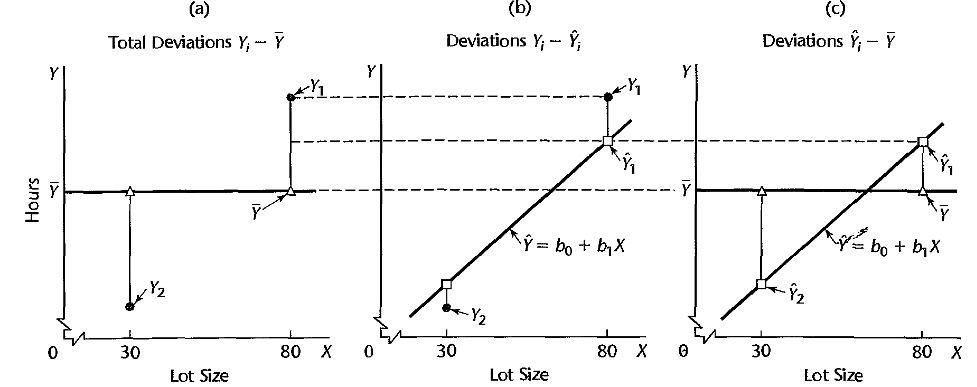
\includegraphics[width=0.65\linewidth]{week2_5} \end{center}
\end{frame}

\begin{frame}{Partition of Total sum of squares}
\protect\hypertarget{partition-of-total-sum-of-squares-1}{}
\begin{itemize}
\item
  Total sum of squares (\(SST\)): \(SST=\sum(y_i-\bar{y})^2.\)
\item
  Error sum of squares (\(SSE\)): \(SSE=\sum (y_i-\hat{y}_i)^2.\)
\item
  Regression sum of squares (\(SSR\)):
  \(SSR=\sum (\hat{y}_i-\bar{y})^2\)
\end{itemize}

Then we have the following relation:
\[\sum(y_i-\bar{y})^2=\sum (\hat{y}_i-\bar{y})^2+\sum (y_i-\hat{y}_i)^2\]
That is: \(SST=SSR+SSE\)
\end{frame}

\begin{frame}{Coefficient of Determination}
\protect\hypertarget{coefficient-of-determination}{}
A natural measure of the effect of \(x\) in reducing in variation in
\(y\) is to express the reduction in variation as a proportion of the
total variation: \[R^2=\frac{SSR}{SST}=1-\frac{SSE}{SST}.\]

We can also write:

\[R^2=\frac{var(\hat{y})}{var(y)}\]

Note that: \[0\leq R^2 \leq 1\]
\end{frame}

\begin{frame}{Coefficient of Determination}
\protect\hypertarget{coefficient-of-determination-1}{}
Some common misunderstandings of \(R^2\):

\begin{itemize}
\item
  A high coefficient of determination indicates that useful predictions
  can be made (not always).
\item
  A high coefficient of determination indicates the estimated regression
  line is a good fit (not always).
\item
  A coefficient of determination near zero indicates that \(x\) and
  \(y\) are not related (not always).
\end{itemize}
\end{frame}

\begin{frame}{Coefficient of Determination}
\protect\hypertarget{coefficient-of-determination-2}{}
\begin{center}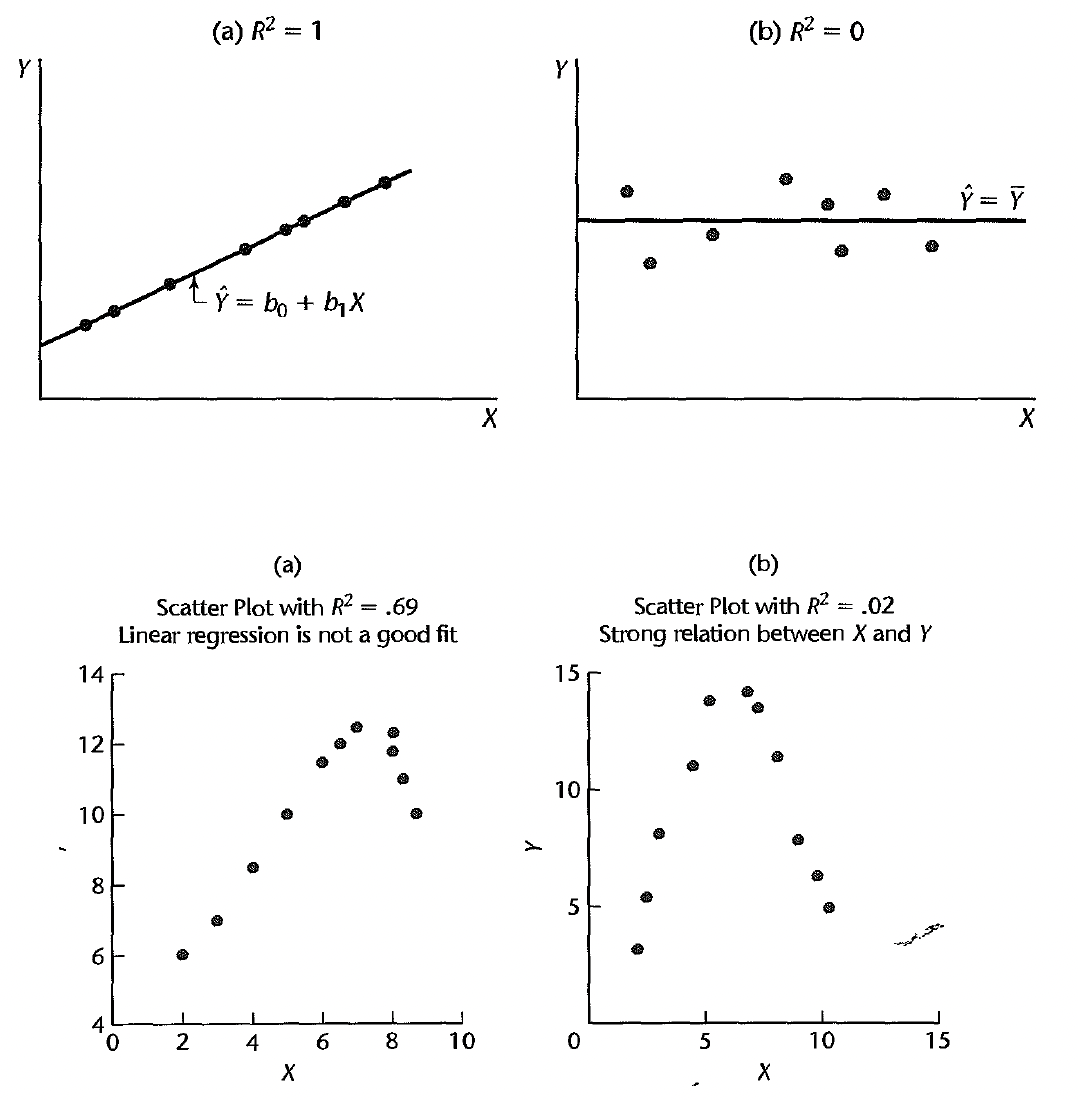
\includegraphics[width=0.6\linewidth]{week2_7} \end{center}
\end{frame}

\begin{frame}[fragile]{Regression: Teaching Evaluations Example}
\protect\hypertarget{regression-teaching-evaluations-example-14}{}
\normalsize

\begin{Shaded}
\begin{Highlighting}[]
\NormalTok{TSS }\OtherTok{\textless{}{-}} \FunctionTok{sum}\NormalTok{((evals\_ch5}\SpecialCharTok{$}\NormalTok{score }\SpecialCharTok{{-}} \FunctionTok{mean}\NormalTok{(evals\_ch5}\SpecialCharTok{$}\NormalTok{score))}\SpecialCharTok{\^{}}\DecValTok{2}\NormalTok{)}
\FunctionTok{c}\NormalTok{(RSS, TSS)}
\end{Highlighting}
\end{Shaded}

\begin{verbatim}
[1] 131.8684 136.6543
\end{verbatim}

\begin{Shaded}
\begin{Highlighting}[]
\NormalTok{R2 }\OtherTok{\textless{}{-}}\NormalTok{ (TSS }\SpecialCharTok{{-}}\NormalTok{ RSS)}\SpecialCharTok{/}\NormalTok{TSS}
\NormalTok{R2}
\end{Highlighting}
\end{Shaded}

\begin{verbatim}
[1] 0.03502226
\end{verbatim}

\begin{Shaded}
\begin{Highlighting}[]
\CommentTok{\# Or}
\FunctionTok{summary}\NormalTok{(score\_model)}\SpecialCharTok{$}\NormalTok{r.squared}
\end{Highlighting}
\end{Shaded}

\begin{verbatim}
[1] 0.03502226
\end{verbatim}

\normalsize
\end{frame}

\begin{frame}[fragile]{Regression: Teaching Evaluations Example}
\protect\hypertarget{regression-teaching-evaluations-example-15}{}
\normalsize

\begin{Shaded}
\begin{Highlighting}[]
\FunctionTok{get\_regression\_points}\NormalTok{(score\_model) }
\end{Highlighting}
\end{Shaded}

\begin{verbatim}
# A tibble: 463 x 5
      ID score bty_avg score_hat residual
   <int> <dbl>   <dbl>     <dbl>    <dbl>
 1     1   4.7    5         4.21    0.486
 2     2   4.1    5         4.21   -0.114
 3     3   3.9    5         4.21   -0.314
 4     4   4.8    5         4.21    0.586
 5     5   4.6    3         4.08    0.52 
 6     6   4.3    3         4.08    0.22 
 7     7   2.8    3         4.08   -1.28 
 8     8   4.1    3.33      4.10   -0.002
 9     9   3.4    3.33      4.10   -0.702
10    10   4.5    3.17      4.09    0.409
# i 453 more rows
\end{verbatim}
\end{frame}

\begin{frame}[fragile]{Regression: Teaching Evaluations Example}
\protect\hypertarget{regression-teaching-evaluations-example-16}{}
\small

\begin{Shaded}
\begin{Highlighting}[]
\FunctionTok{get\_regression\_points}\NormalTok{(score\_model) }\SpecialCharTok{|\textgreater{}} 
  \FunctionTok{summarize}\NormalTok{(}\AttributeTok{var\_y =} \FunctionTok{var}\NormalTok{(score), }
            \AttributeTok{var\_y\_hat =} \FunctionTok{var}\NormalTok{(score\_hat), }
            \AttributeTok{var\_residual =} \FunctionTok{var}\NormalTok{(residual)) }\SpecialCharTok{|\textgreater{}} 
  \FunctionTok{mutate}\NormalTok{(}\AttributeTok{R2 =}\NormalTok{ var\_y\_hat}\SpecialCharTok{/}\NormalTok{var\_y)}
\end{Highlighting}
\end{Shaded}

\begin{verbatim}
# A tibble: 1 x 4
  var_y var_y_hat var_residual     R2
  <dbl>     <dbl>        <dbl>  <dbl>
1 0.296    0.0104        0.285 0.0350
\end{verbatim}
\end{frame}

\hypertarget{prediction-intervals}{%
\section{Prediction intervals}\label{prediction-intervals}}

\begin{frame}{Interval Estimation for Mean Response and a Single
Response}
\protect\hypertarget{interval-estimation-for-mean-response-and-a-single-response}{}
\begin{enumerate}
\tightlist
\item
  Estimating the mean of \(y\) at a given value of \(x\), that is,
  \(E(y|x)=\mu_{y|x}\)
\end{enumerate}

\textbf{Example}: A power company may want to estimate the mean daily
power consumption for a given temperature. They need this estimate for a
report.

\begin{enumerate}
\setcounter{enumi}{1}
\tightlist
\item
  Predicting a single value of \(y\) for a given value of \(x\).
\end{enumerate}

\textbf{Example}: The power company want to predict power consumption on
a single day for a given temperature.

\begin{itemize}
\item
  They might know a hot day is coming up the next day and have good idea
  of what the high temperature will be, so what to predict the power
  consumption.
\item
  We want to be \(99.99\%\) confident that they have enough access to
  power to cover demand.
\end{itemize}
\end{frame}

\begin{frame}{Interval Estimation of Mean Response}
\protect\hypertarget{interval-estimation-of-mean-response}{}
Let \(x_h\) denote the level of \(x\) for which we wish to estimate the
mean response. Then, by the regression equation we have:
\[E(y_h|x_h)=\hat{y}_h=b_0+b_1x_h\] Variance:

\[Var(\hat{y}_h)=\sigma^2\left[\frac{1}{n}+\frac{(x_h-\bar{x})^2}{\Sigma(x_i-\bar{x})^2}\right]\]

Estimated Variance:
\[S^2(\hat{y}_h)=MSE\left[\frac{1}{n}+\frac{(x_h-\bar{x})^2}{\Sigma(x_i-\bar{x})^2}\right]\]
\end{frame}

\begin{frame}{Interval Estimation of Mean Response}
\protect\hypertarget{interval-estimation-of-mean-response-1}{}
\begin{itemize}
\tightlist
\item
  \(t-\)distribution
\end{itemize}

\[\frac{y_h-\hat{y}_h}{S(\hat{y}_h)}\sim t_{n-2}\]

So, the \(100(1-\alpha)\%\) confidence interval for the mean response
is: \[\hat{y}_h\pm t_{1 -\alpha/2; n-2}S(\hat{y}_h).\]
\end{frame}

\begin{frame}{Prediction Intervals for a Single Response}
\protect\hypertarget{prediction-intervals-for-a-single-response}{}
In prediction of a single response, we can use the estimated mean
function to predict it. Let \(x_*\) denote the level of \(x\), then we
have:
\[ y_*=\beta_0+\beta_1x_*+\epsilon_*, \quad \quad Var(\epsilon_*)=\sigma^2.\]
A natural estimation is: \[ \hat{y}_*=b_0+b_1x_*.\]

\begin{itemize}
\tightlist
\item
  The variance of prediction error:
  \[ Var(pred)=\sigma^2+\sigma^2\left(\frac{1}{n}+\frac{(x_* -\bar{x})^2}{\sum (x_* -\bar{x})^2}\right)\]
\item
  The estimated standard error of prediction at \(x_*\):
  \[S(pred)=\sqrt{MSE}\left(1+\frac{1}{n}+\frac{(x_* -\bar{x})^2}{\sum (x_* -\bar{x})^2}\right)\]
\end{itemize}
\end{frame}

\begin{frame}{Prediction Intervals for a Single Response}
\protect\hypertarget{prediction-intervals-for-a-single-response-1}{}
Hence,

\[\frac{y_*-\hat{y}_*}{S(pred)}\sim t_{n-2}.\]

So, the prediction interval for \(y_*\) is:
\[\hat{y}_*\pm t_{1 - \alpha/2; n-2}S(pred).\]
\end{frame}

\begin{frame}[fragile]{Confidence Regions and Prediction Bands}
\protect\hypertarget{confidence-regions-and-prediction-bands}{}
\begin{Shaded}
\begin{Highlighting}[]
\NormalTok{PIM }\OtherTok{\textless{}{-}} \FunctionTok{predict}\NormalTok{(score\_model, }\AttributeTok{interval =} \StringTok{"pred"}\NormalTok{)}
\NormalTok{df1 }\OtherTok{\textless{}{-}} \FunctionTok{cbind}\NormalTok{(evals\_ch5, PIM)}
\FunctionTok{ggplot}\NormalTok{(}\AttributeTok{data =}\NormalTok{ df1, }\FunctionTok{aes}\NormalTok{(}\AttributeTok{x =}\NormalTok{ bty\_avg, }\AttributeTok{y =}\NormalTok{ score)) }\SpecialCharTok{+} 
  \FunctionTok{geom\_point}\NormalTok{() }\SpecialCharTok{+} 
  \FunctionTok{geom\_smooth}\NormalTok{(}\AttributeTok{method =} \StringTok{"lm"}\NormalTok{) }\SpecialCharTok{+} 
  \FunctionTok{geom\_line}\NormalTok{(}\FunctionTok{aes}\NormalTok{(}\AttributeTok{y =}\NormalTok{ upr), }\AttributeTok{color =} \StringTok{"purple"}\NormalTok{, }
            \AttributeTok{linetype =} \StringTok{"dashed"}\NormalTok{) }\SpecialCharTok{+} 
  \FunctionTok{geom\_line}\NormalTok{(}\FunctionTok{aes}\NormalTok{(}\AttributeTok{y =}\NormalTok{ lwr), }\AttributeTok{color =} \StringTok{"purple"}\NormalTok{, }
            \AttributeTok{linetype =} \StringTok{"dashed"}\NormalTok{) }\SpecialCharTok{+} 
  \FunctionTok{theme\_bw}\NormalTok{() }\OtherTok{{-}\textgreater{}}\NormalTok{ p1}
\NormalTok{p1}
\end{Highlighting}
\end{Shaded}
\end{frame}

\begin{frame}{Confidence Regions and Prediction Bands}
\protect\hypertarget{confidence-regions-and-prediction-bands-1}{}
\begin{center}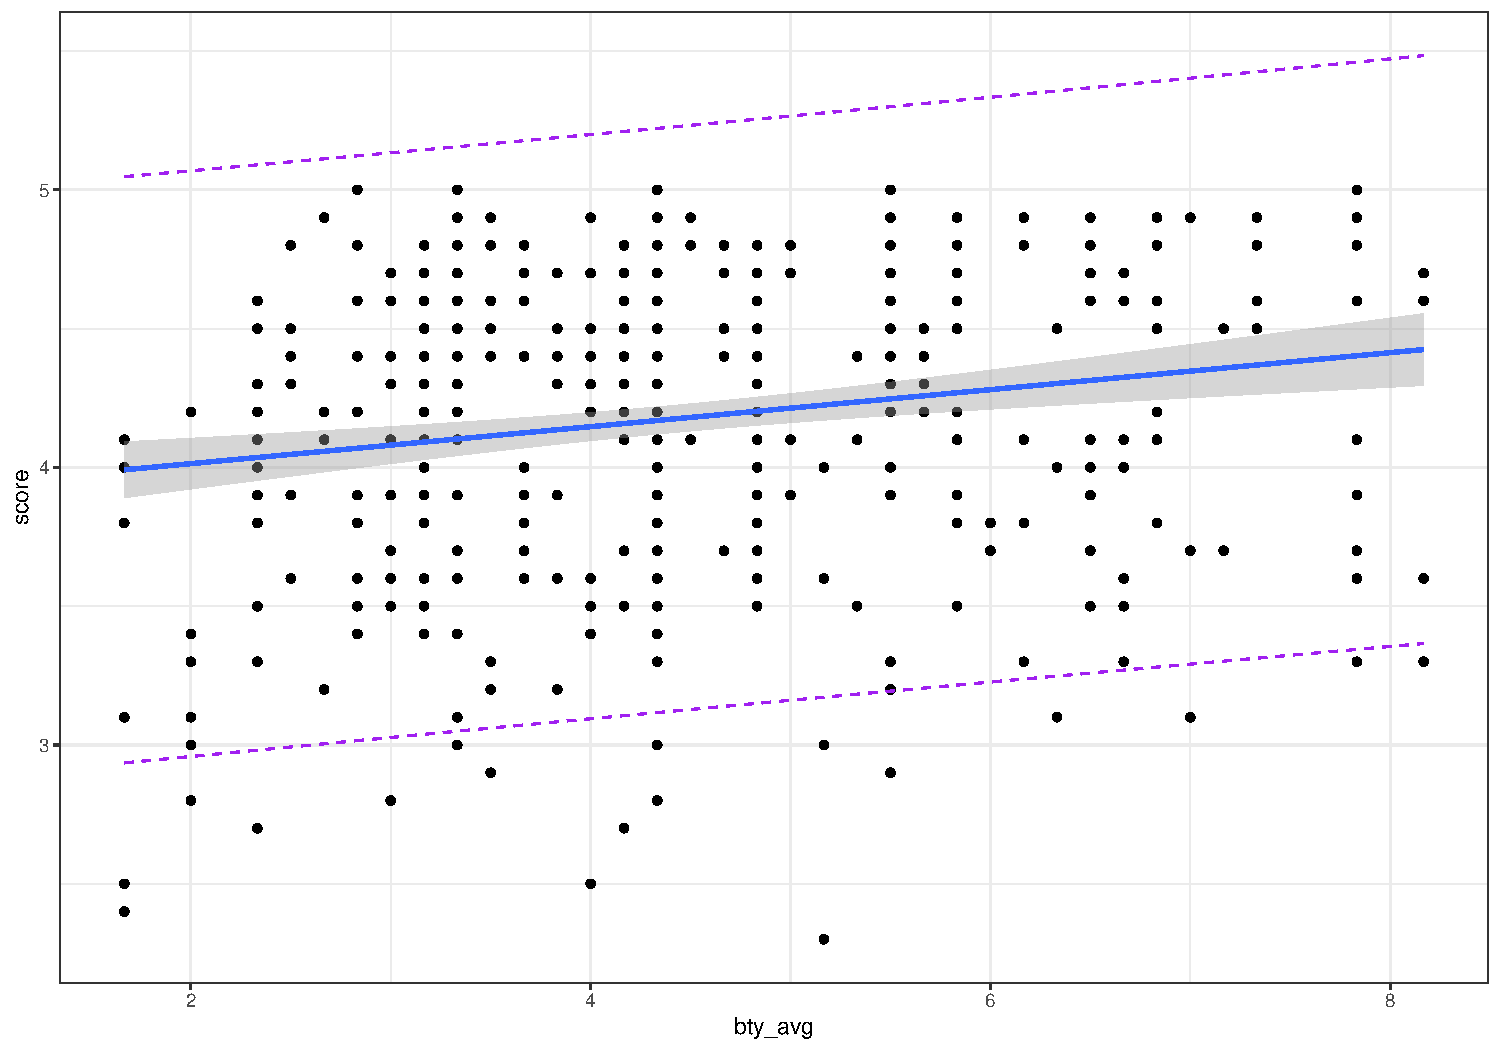
\includegraphics[width=0.7\linewidth,height=0.7\textheight]{Week4_Int_Lect_files/figure-beamer/unnamed-chunk-40-1} \end{center}
\end{frame}

\begin{frame}[fragile]{Regression: Teaching Evaluations Example}
\protect\hypertarget{regression-teaching-evaluations-example-17}{}
\normalsize

\begin{Shaded}
\begin{Highlighting}[]
\CommentTok{\# Using the build in function}
\FunctionTok{predict}\NormalTok{(score\_model, }\AttributeTok{newdata =} \FunctionTok{data.frame}\NormalTok{(}\AttributeTok{bty\_avg =} \FloatTok{7.333}\NormalTok{))}
\end{Highlighting}
\end{Shaded}

\begin{verbatim}
       1 
4.368987 
\end{verbatim}

\begin{Shaded}
\begin{Highlighting}[]
\CommentTok{\# 90\% Confidence Interval for E(Y\_7.333)}
\FunctionTok{predict}\NormalTok{(score\_model, }\AttributeTok{newdata =} \FunctionTok{data.frame}\NormalTok{(}\AttributeTok{bty\_avg =} \FloatTok{7.333}\NormalTok{), }
        \AttributeTok{interval =} \StringTok{"conf"}\NormalTok{, }\AttributeTok{level =} \FloatTok{0.90}\NormalTok{)}
\end{Highlighting}
\end{Shaded}

\begin{verbatim}
       fit      lwr      upr
1 4.368987 4.280641 4.457333
\end{verbatim}

\begin{Shaded}
\begin{Highlighting}[]
\CommentTok{\# 90\% Prediction Interval for Y\_hat\_7.333}
\FunctionTok{predict}\NormalTok{(score\_model, }\AttributeTok{newdata =} \FunctionTok{data.frame}\NormalTok{(}\AttributeTok{bty\_avg =} \FloatTok{7.333}\NormalTok{), }
        \AttributeTok{interval =} \StringTok{"pred"}\NormalTok{, }\AttributeTok{level =} \FloatTok{0.90}\NormalTok{)}
\end{Highlighting}
\end{Shaded}

\begin{verbatim}
       fit      lwr    upr
1 4.368987 3.483074 5.2549
\end{verbatim}

\normalsize
\end{frame}

\hypertarget{related-topics}{%
\section{Related topics}\label{related-topics}}

\begin{frame}[fragile]{Correlation is not necessarily causation}
\protect\hypertarget{correlation-is-not-necessarily-causation}{}
\begin{itemize}
\item
  Throughout this chapter we've been cautious when interpreting
  regression slope coefficients.

  \begin{itemize}
  \tightlist
  \item
    We always discussed the ``associated'' effect of an explanatory
    variable \(x\) on an outcome variable \(y\).
  \item
    We include the term ``associated'' to be extra careful not to
    suggest we are making a \textbf{causal} statement.
  \end{itemize}
\item
  For example when we looked at the teaching score and ``beauty''
  example:

  \begin{itemize}
  \item
    For every increase of 1 unit in \texttt{bty\_avg} there is an
    associated increase of on average 0.067 units for the variable
    \texttt{score}.
  \item
    while \texttt{bty\_avg} is positively correlated with
    \texttt{score}, we can't necessarily make any statements about
    ``beauty'' scores' direct causal effect on teaching score without
    more information on how this study was conducted.
  \end{itemize}
\end{itemize}
\end{frame}

\begin{frame}{Correlation is not necessarily causation}
\protect\hypertarget{correlation-is-not-necessarily-causation-1}{}
Here is another example:

\begin{itemize}
\item
  A not-so-great medical doctor goes through medical records and finds
  that patients who slept with their shoes on tended to wake up more
  with headaches.

  \begin{itemize}
  \tightlist
  \item
    So this doctor declares, ``Sleeping with shoes on causes
    headaches!''
  \end{itemize}
\end{itemize}

\begin{center}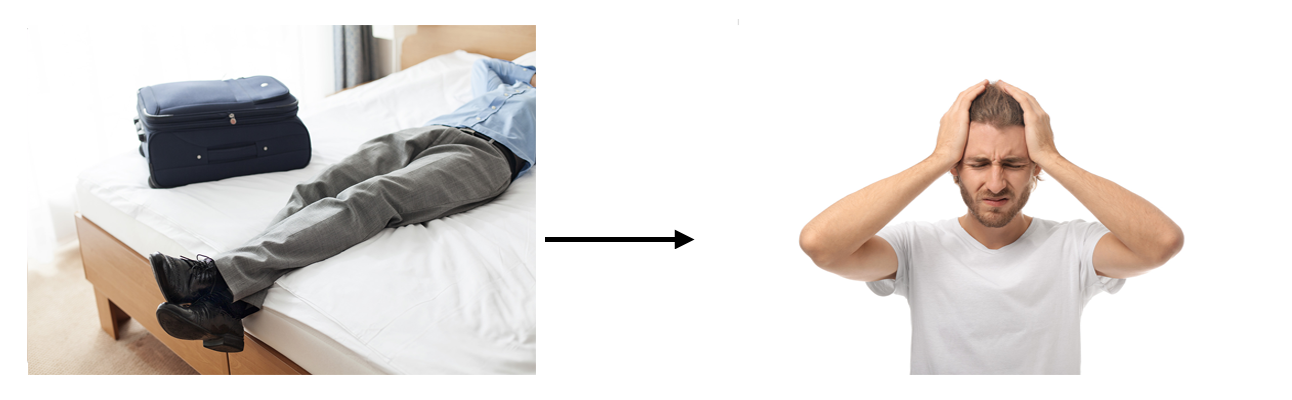
\includegraphics[width=0.8\linewidth,height=0.35\textheight]{week4_7} \end{center}
\end{frame}

\begin{frame}{Correlation is not necessarily causation}
\protect\hypertarget{correlation-is-not-necessarily-causation-2}{}
\begin{itemize}
\item
  However, there is a good chance that if someone is sleeping with their
  shoes on, it's potentially because they are intoxicated from alcohol.

  \begin{itemize}
  \tightlist
  \item
    Higher levels of drinking leads to more hangovers, and hence more
    headaches.
  \item
    The amount of alcohol consumption here is what's known as a
    confounding/lurking variable.
  \item
    It ``lurks'' behind the scenes, confounding the causal relationship
    (if any) of ``sleeping with shoes on'' with ``waking up with a
    headache''.
  \end{itemize}
\end{itemize}

\begin{center}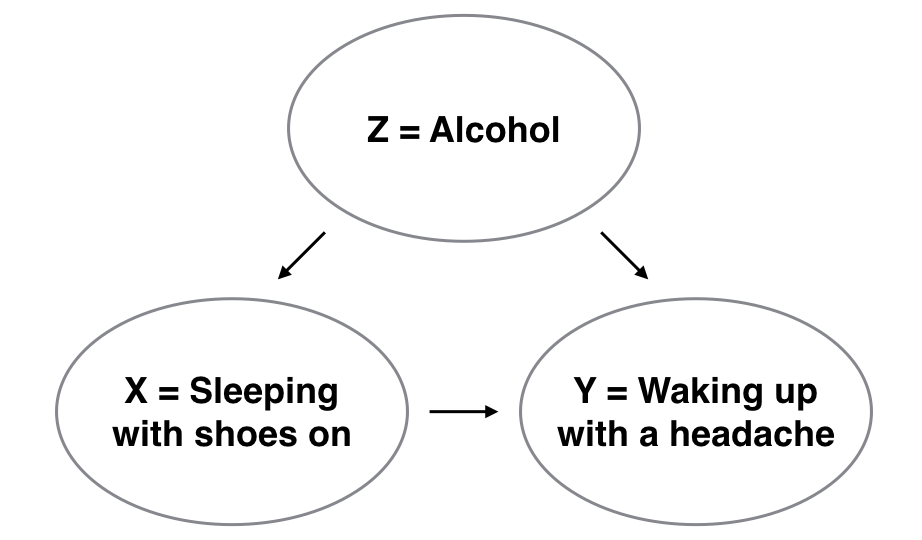
\includegraphics[width=0.6\linewidth,height=0.3\textheight]{week4_8} \end{center}

\(Z\) is a confounding variable.
\end{frame}

\begin{frame}{Correlation is not necessarily causation}
\protect\hypertarget{correlation-is-not-necessarily-causation-3}{}
\begin{itemize}
\item
  Establishing \textbf{causation} is a tricky problem which requires:

  \begin{enumerate}
  \tightlist
  \item
    carefully designed experiments or
  \item
    methods to control for the effects of confounding variables
  \end{enumerate}
\item
  Both these approaches attempt, as best they can, either to take all
  possible confounding variables into account or negate their impact.
\item
  This allows researchers to focus only on the relationship of interest:
  the relationship between the outcome variable \(Y\) and the treatment
  variable \(X\).
\item
  As you read news stories, be careful not to fall into the trap of
  thinking that correlation necessarily implies causation.
\end{itemize}
\end{frame}

\begin{frame}{Best-fitting line}
\protect\hypertarget{best-fitting-line}{}
Regression lines are also known as ``best-fitting'' lines. But what do
we mean by ``best''?

\begin{itemize}
\tightlist
\item
  Lets use the Teaching Evaluations Example.
\end{itemize}

\begin{center}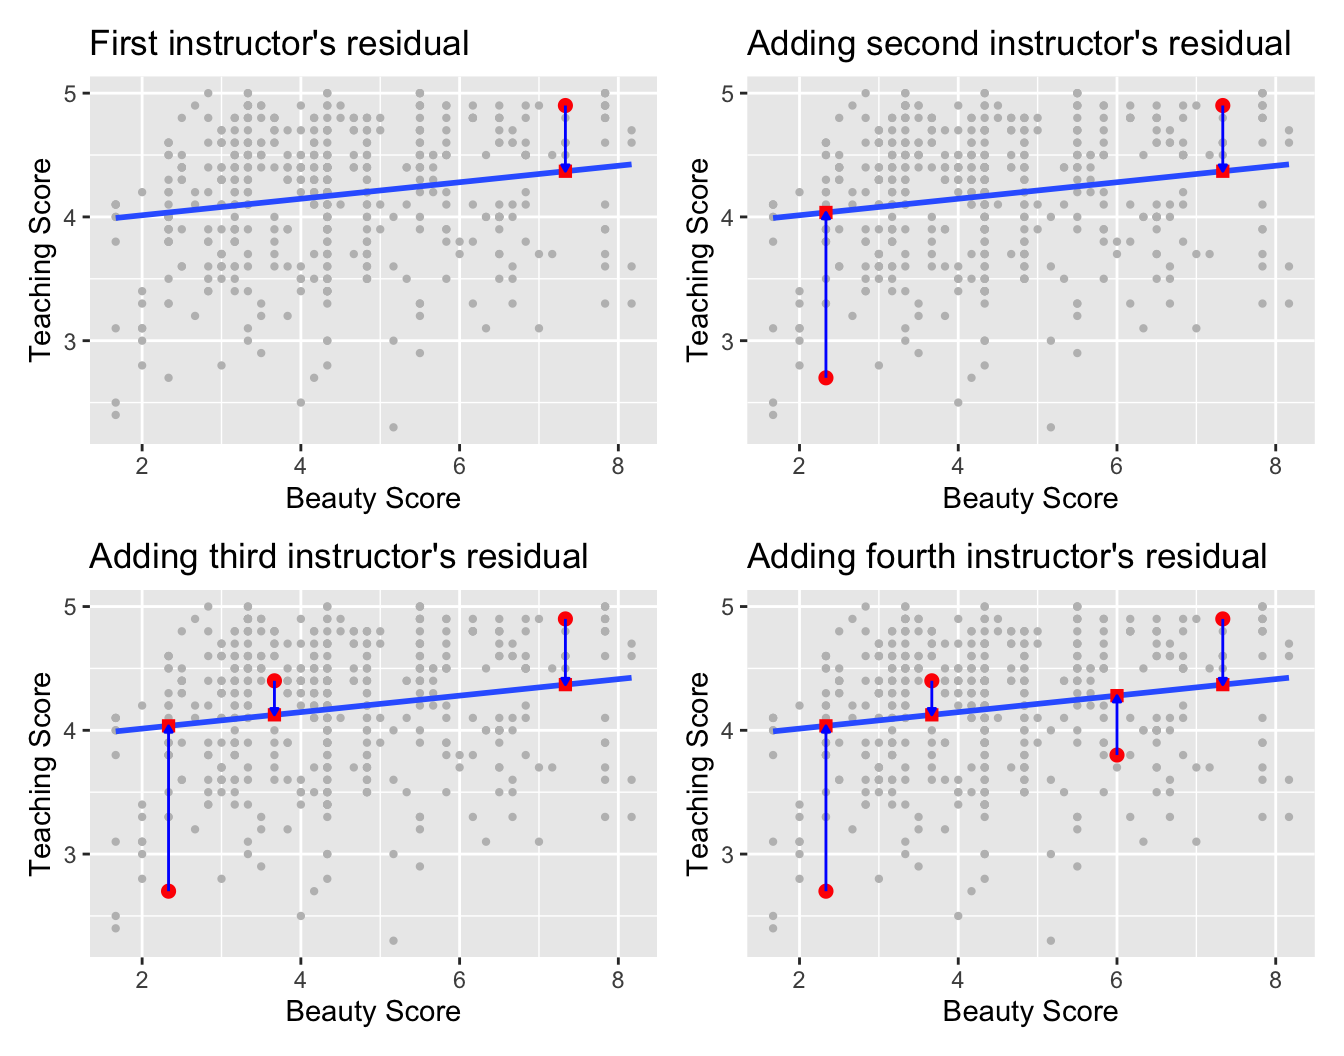
\includegraphics[width=0.8\linewidth,height=0.5\textheight]{week4_9} \end{center}

we mark the observed value \(y\) with a circle, the fitted value
\(\hat{y}\) with a square and the residuals \(y-\hat{y}\) with a
vertical blue line.
\end{frame}

\begin{frame}{Best-fitting line}
\protect\hypertarget{best-fitting-line-1}{}
\begin{itemize}
\item
  Now say we repeated this process of computing residuals for all 463
  courses' instructors,

  \begin{itemize}
  \tightlist
  \item
    then we squared all the residuals, and
  \item
    then we summed them.
  \item
    We call this quantity the sum of squared residuals.
  \end{itemize}
\item
  The \textbf{sum of squared residuals} is a measure of the lack of fit
  of a model.

  \begin{itemize}
  \tightlist
  \item
    Larger values of the sum of squared residuals indicate a bigger lack
    of fit. This corresponds to a worse fitting model.
  \item
    If the regression line fits all the points perfectly, then the sum
    of squared residuals is 0.
  \end{itemize}
\item
  The regression line minimizes the sum of the squared residuals:
  \[\sum_{i=1}^n(y_i-\hat{y}_i)^2\]
\end{itemize}
\end{frame}

\begin{frame}[fragile]{Best-fitting line}
\protect\hypertarget{best-fitting-line-2}{}
\normalsize

\begin{Shaded}
\begin{Highlighting}[]
\CommentTok{\# Fit regression model:}
\NormalTok{score\_model }\OtherTok{\textless{}{-}} \FunctionTok{lm}\NormalTok{(score }\SpecialCharTok{\textasciitilde{}}\NormalTok{ bty\_avg, }\AttributeTok{data =}\NormalTok{ evals\_ch5)}
\CommentTok{\# Get regression points:}
\NormalTok{regression\_points }\OtherTok{\textless{}{-}} \FunctionTok{get\_regression\_points}\NormalTok{(score\_model)}
\FunctionTok{head}\NormalTok{(regression\_points)}
\end{Highlighting}
\end{Shaded}

\begin{verbatim}
# A tibble: 6 x 5
     ID score bty_avg score_hat residual
  <int> <dbl>   <dbl>     <dbl>    <dbl>
1     1   4.7       5      4.21    0.486
2     2   4.1       5      4.21   -0.114
3     3   3.9       5      4.21   -0.314
4     4   4.8       5      4.21    0.586
5     5   4.6       3      4.08    0.52 
6     6   4.3       3      4.08    0.22 
\end{verbatim}

\normalsize
\end{frame}

\begin{frame}[fragile]{Best-fitting line}
\protect\hypertarget{best-fitting-line-3}{}
Any other straight line drawn in the figure would yield a sum of squared
residuals greater than 132.

\normalsize

\begin{Shaded}
\begin{Highlighting}[]
\CommentTok{\# Compute sum of squared residuals}
\NormalTok{regression\_points }\SpecialCharTok{|\textgreater{}}
  \FunctionTok{mutate}\NormalTok{(}\AttributeTok{squared\_residuals =}\NormalTok{ residual}\SpecialCharTok{\^{}}\DecValTok{2}\NormalTok{) }\SpecialCharTok{|\textgreater{}}
  \FunctionTok{summarize}\NormalTok{(}\AttributeTok{sum\_of\_squared\_residuals =} \FunctionTok{sum}\NormalTok{(squared\_residuals))}
\end{Highlighting}
\end{Shaded}

\begin{verbatim}
# A tibble: 1 x 1
  sum_of_squared_residuals
                     <dbl>
1                     132.
\end{verbatim}

\normalsize
\end{frame}

\begin{frame}[fragile]{Best-fitting line}
\protect\hypertarget{best-fitting-line-4}{}
You can also get the residuals using the function \texttt{resid} on a
linear model object.

\normalsize

\begin{Shaded}
\begin{Highlighting}[]
\CommentTok{\# Compute sum of squared residuals}
\NormalTok{eis }\OtherTok{\textless{}{-}} \FunctionTok{resid}\NormalTok{(score\_model)}
\NormalTok{RSS }\OtherTok{\textless{}{-}} \FunctionTok{sum}\NormalTok{(eis}\SpecialCharTok{\^{}}\DecValTok{2}\NormalTok{)}
\NormalTok{RSS}
\end{Highlighting}
\end{Shaded}

\begin{verbatim}
[1] 131.8684
\end{verbatim}

\begin{Shaded}
\begin{Highlighting}[]
\CommentTok{\# or}
\FunctionTok{anova}\NormalTok{(score\_model)[}\DecValTok{2}\NormalTok{, }\DecValTok{2}\NormalTok{]}
\end{Highlighting}
\end{Shaded}

\begin{verbatim}
[1] 131.8684
\end{verbatim}

\normalsize
\end{frame}

\end{document}
